\chapter{Results and Interpretation}
\label{chap:results}

The background estimation techniques described in the previous chapters are used to make predictions
in each of the 282 signal regions bins. We then compare and fit to observed event counts, using a
maximum-likelihood fit that takes into account all statistical and systematic uncertainties.
Finally, the results of this fit are used to constrain a variety of BSM physics
scenarios.
All results are published in Ref.~\cite{CMS:mt2fullrun2}.
 Sec.~\ref{sec:prefit} presents the raw, pre-fit results, Sec.~\ref{sec:fits} briefly describes
the fitting and limit-setting procedures, and Sec.~\ref{sec:interp} shows
the resulting limits placed on all considered signal models.

\section{Pre-fit results}
\label{sec:prefit}

Figures~\ref{fig:results_mono_vl} to \ref{fig:results_incl} show comparisons of the pre-fit background estimates
and observed yields in all signal regions. The hatched regions in the upper panels (and the solid gray bands
in the ratio panels) represent the total statistical and systematic uncertainty in the background prediction.
For the monojet region, the $x$ axis binning is $\pt^\mrm{jet1}$ (in\GeV), and for the $\Nj\geq2$ regions
the $x$ axis binning is \mttwo (in\GeV). Dashed lines separate the bins into categories of \Nj and \Nb.
Observed yields are statistically consistent with the estimated SM background.

\begin{figure}[htbp]
  \begin{center}
    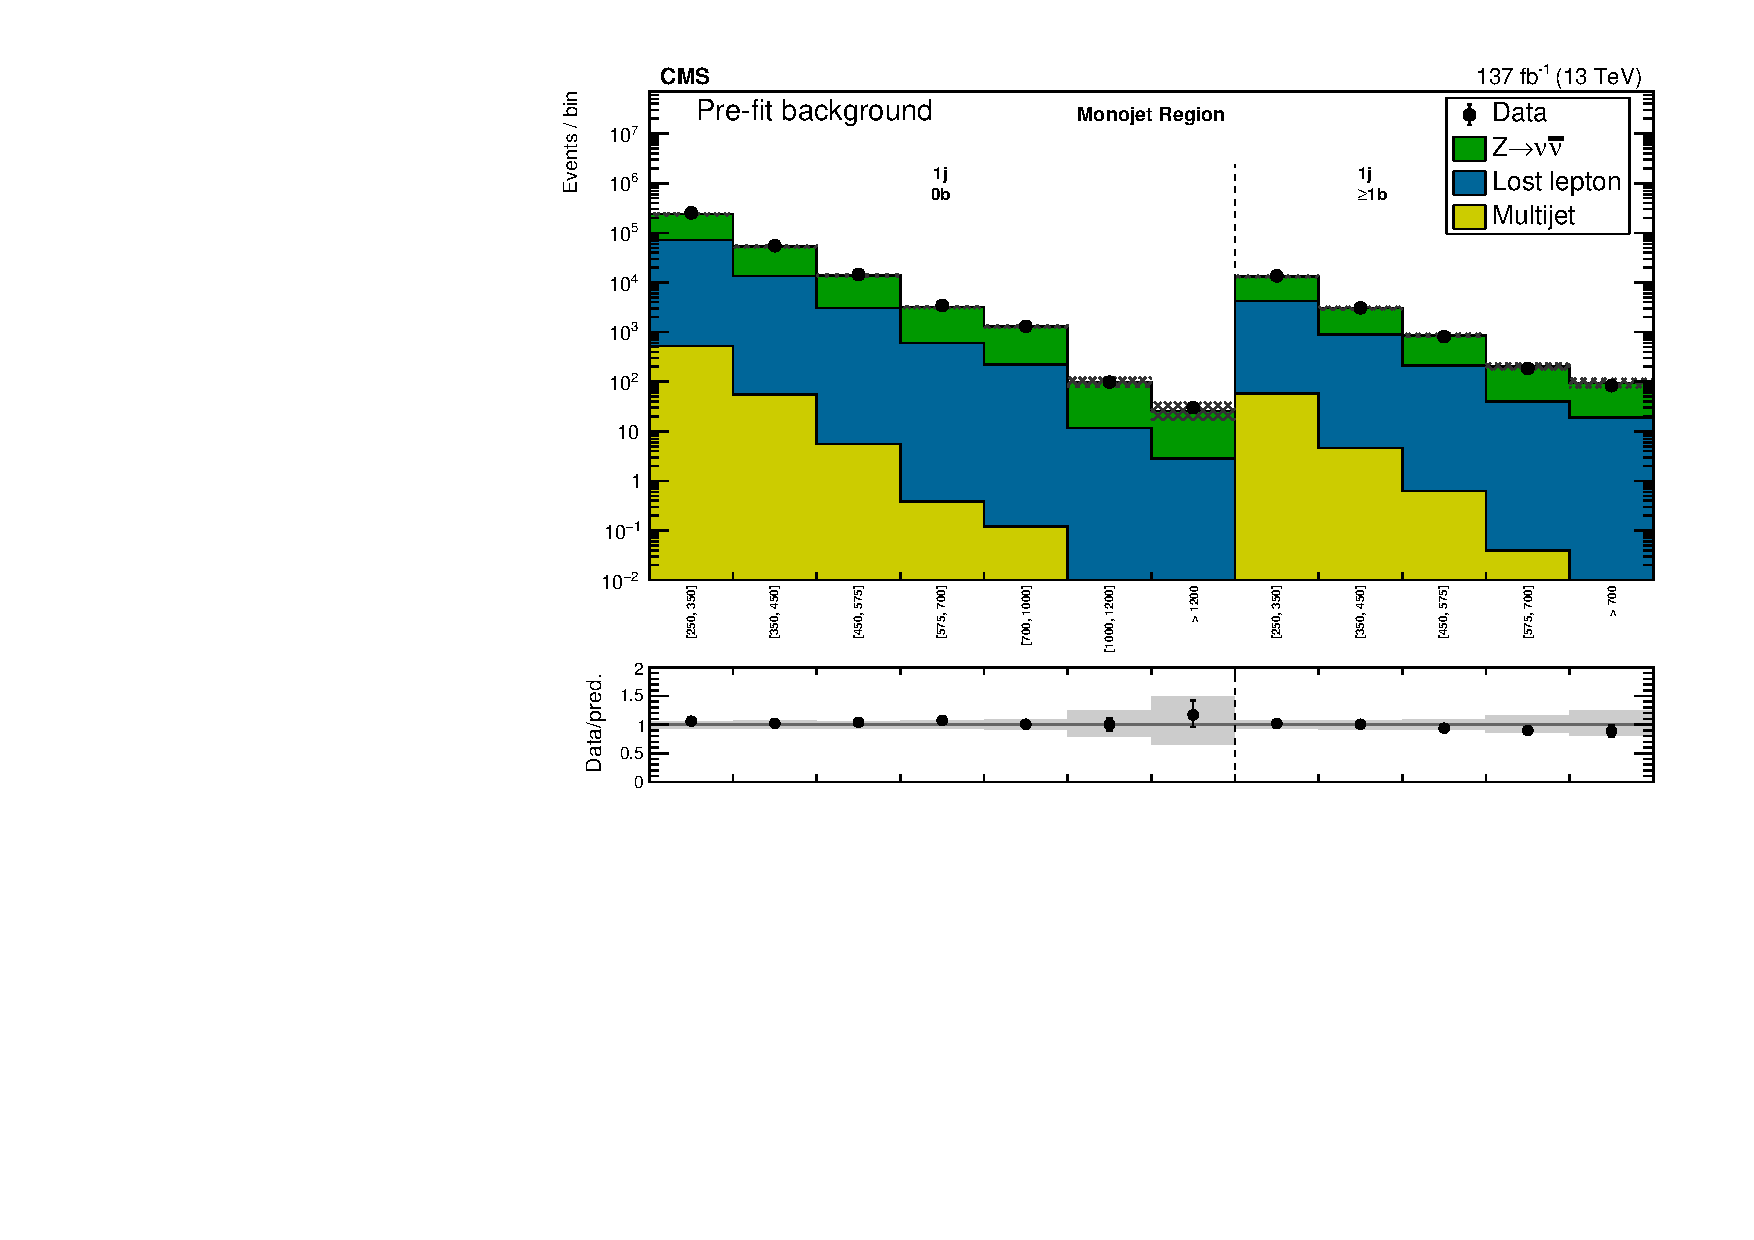
\includegraphics[width=0.93\textwidth]{figs/results/prefit_monojet_ratio.pdf} \\
    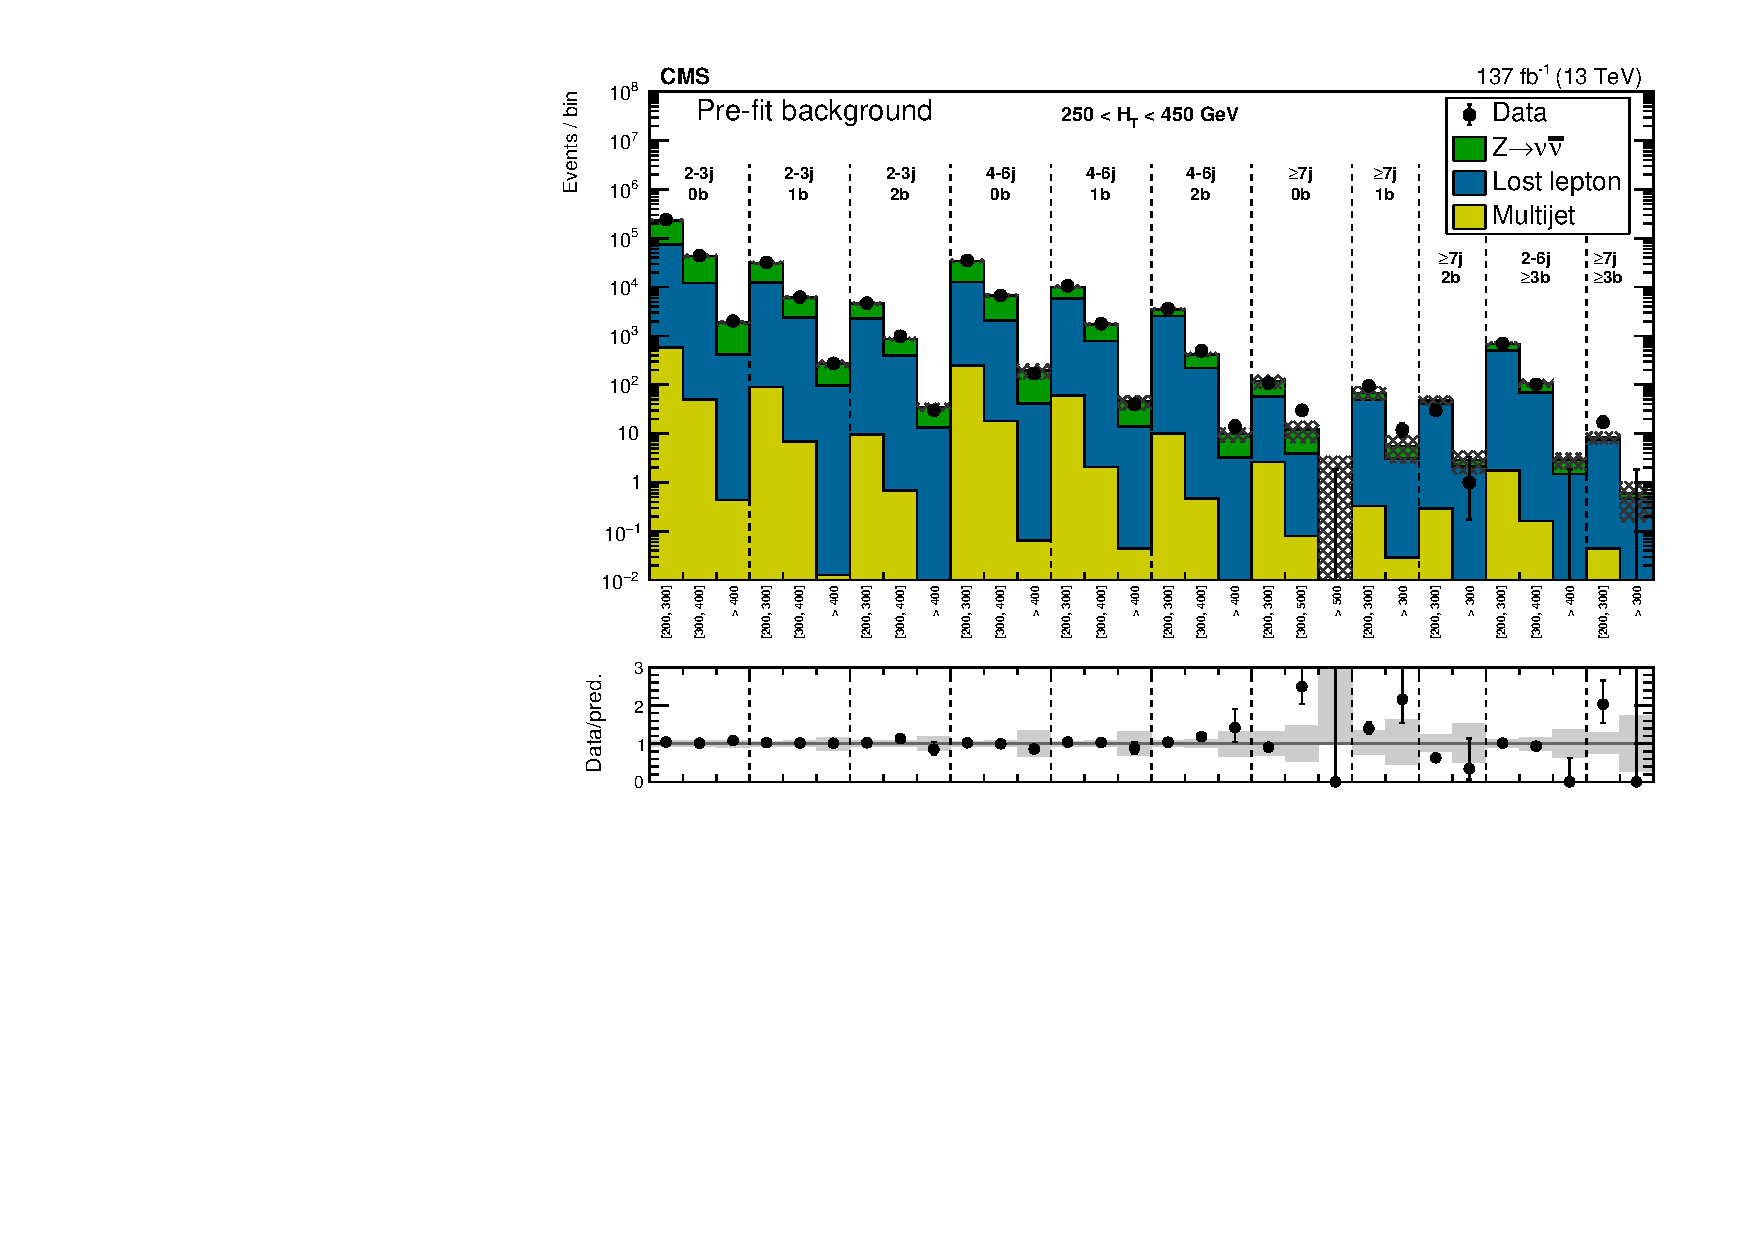
\includegraphics[width=0.93\textwidth]{figs/results/prefit_HT250to450_ratio.pdf} \\
    \caption{Expected (pre-fit) and observed yields for the full data set collected from
      2016--18, corresponding to an integrated luminosity of \Lint. On top are the monojet
      signal regions, separated into \Nb categories and with $\pt^\mrm{jet1}$ binning on the $x$ axis.
      On the bottom are the $\Nj\geq2$ signal regions with $250 \leq \Ht < 450\GeV$, separated into
      topological regions with the \mttwo binning on the $x$ axis.
            }
    \label{fig:results_mono_vl}
  \end{center}
\end{figure}

\begin{figure}[htbp]
  \begin{center}
    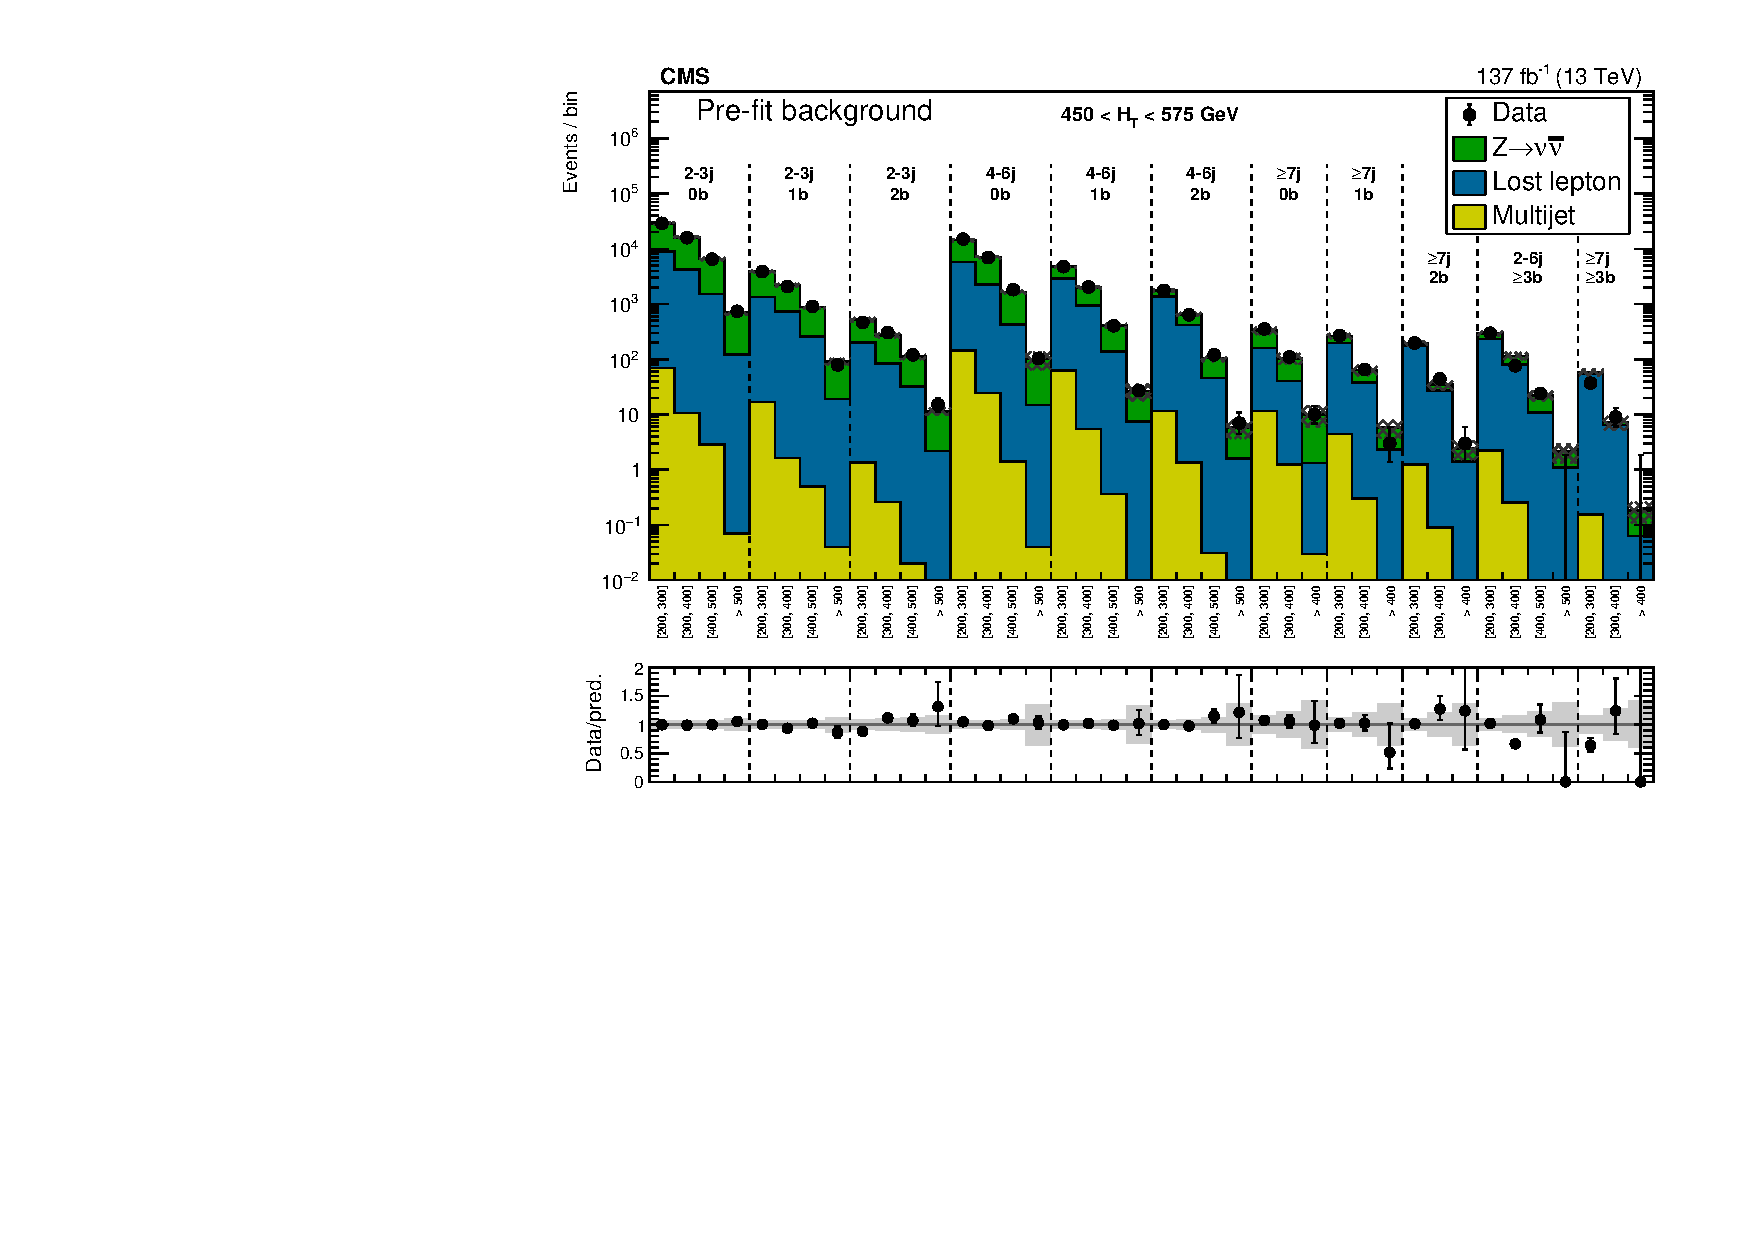
\includegraphics[width=0.93\textwidth]{figs/results/prefit_HT450to575_ratio.pdf} \\
    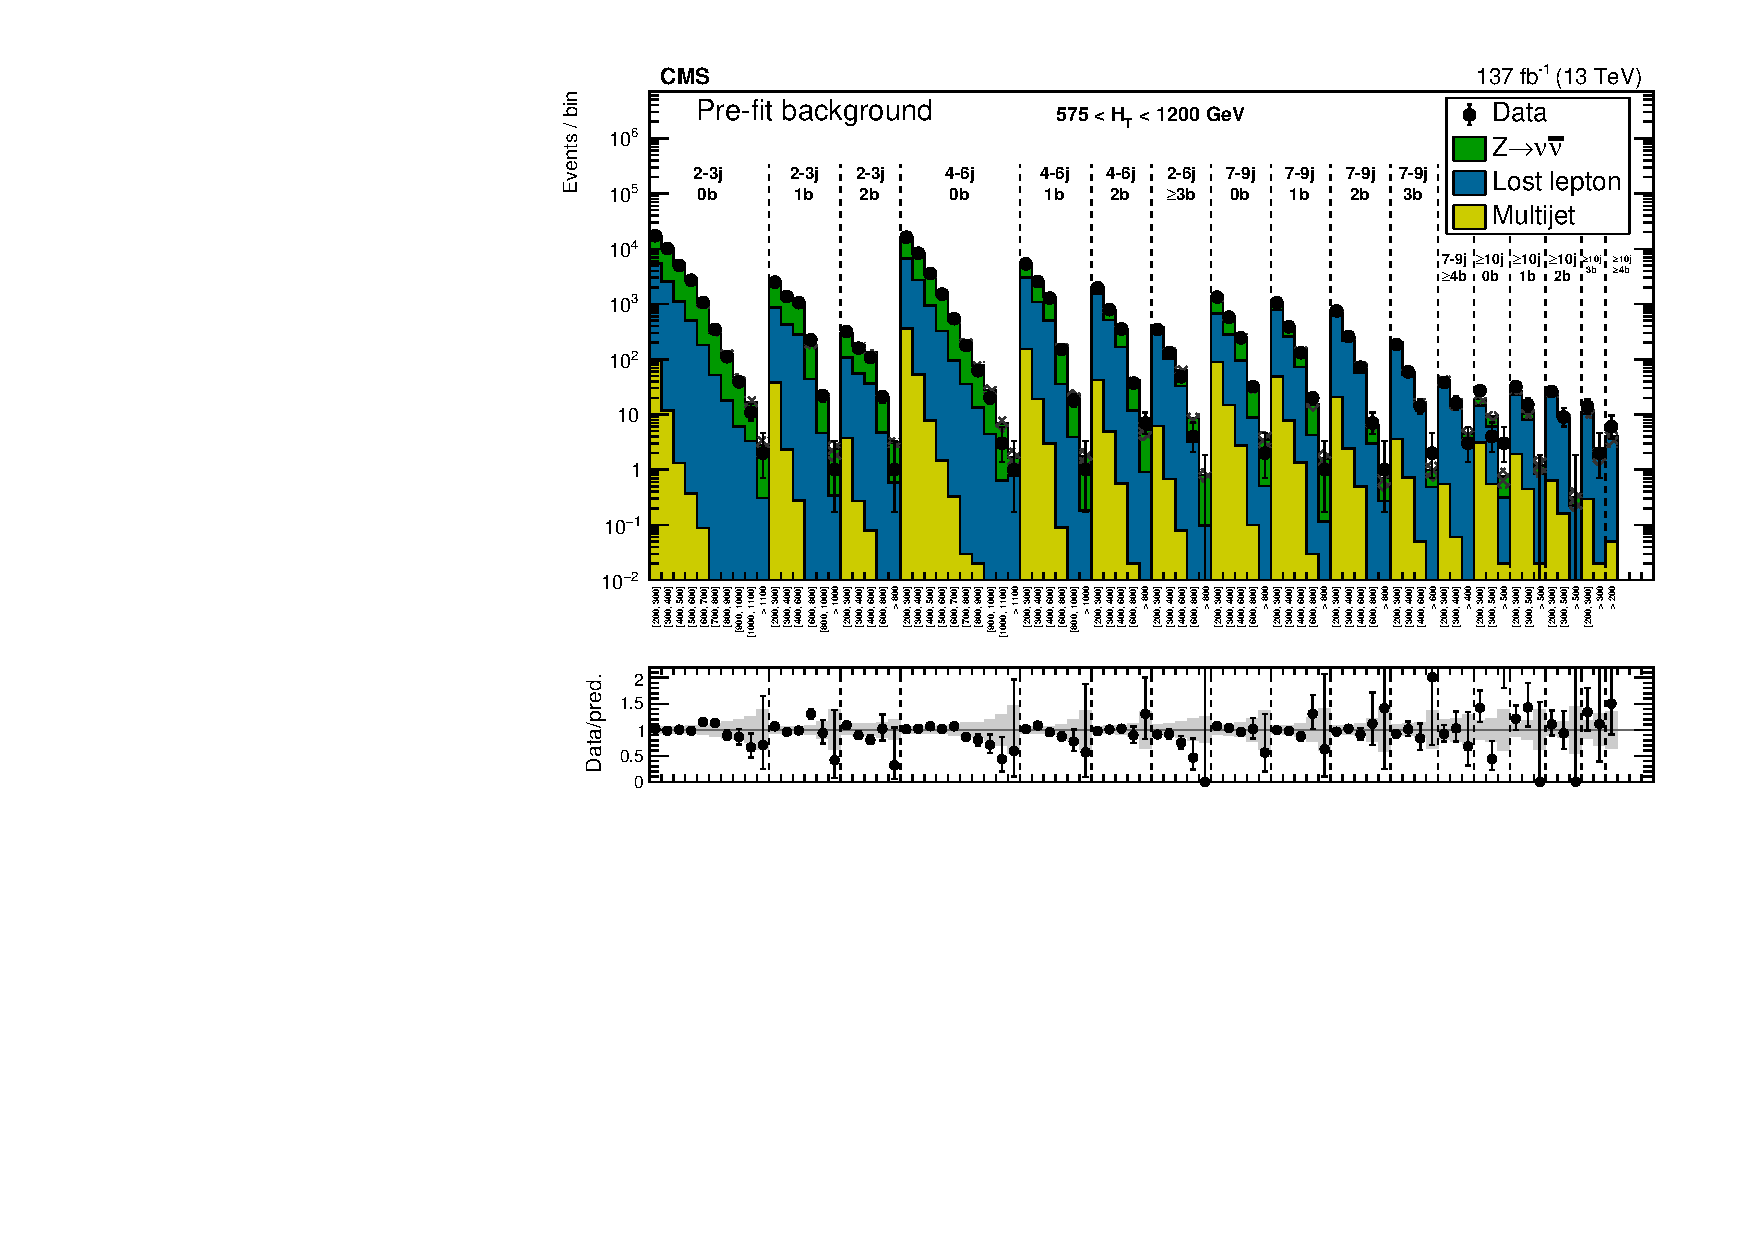
\includegraphics[width=0.93\textwidth]{figs/results/prefit_HT575to1200_ratio.pdf} \\
    \caption{Expected (pre-fit) and observed yields for the full data set collected from
      2016--18, corresponding to an integrated luminosity of \Lint. The top and bottom figures
      contain the $\Nj\geq2$ signal regions for the $450 \leq \Ht < 575\GeV$ and $575 \leq \Ht < 1200\GeV$
      regions, respectively. \mttwo binning is shown on the $x$ axis, with the dashed lines separating
      bins by topological region.
            }
    \label{fig:results_l_m}
  \end{center}
\end{figure}

\begin{figure}[htbp]
  \begin{center}
    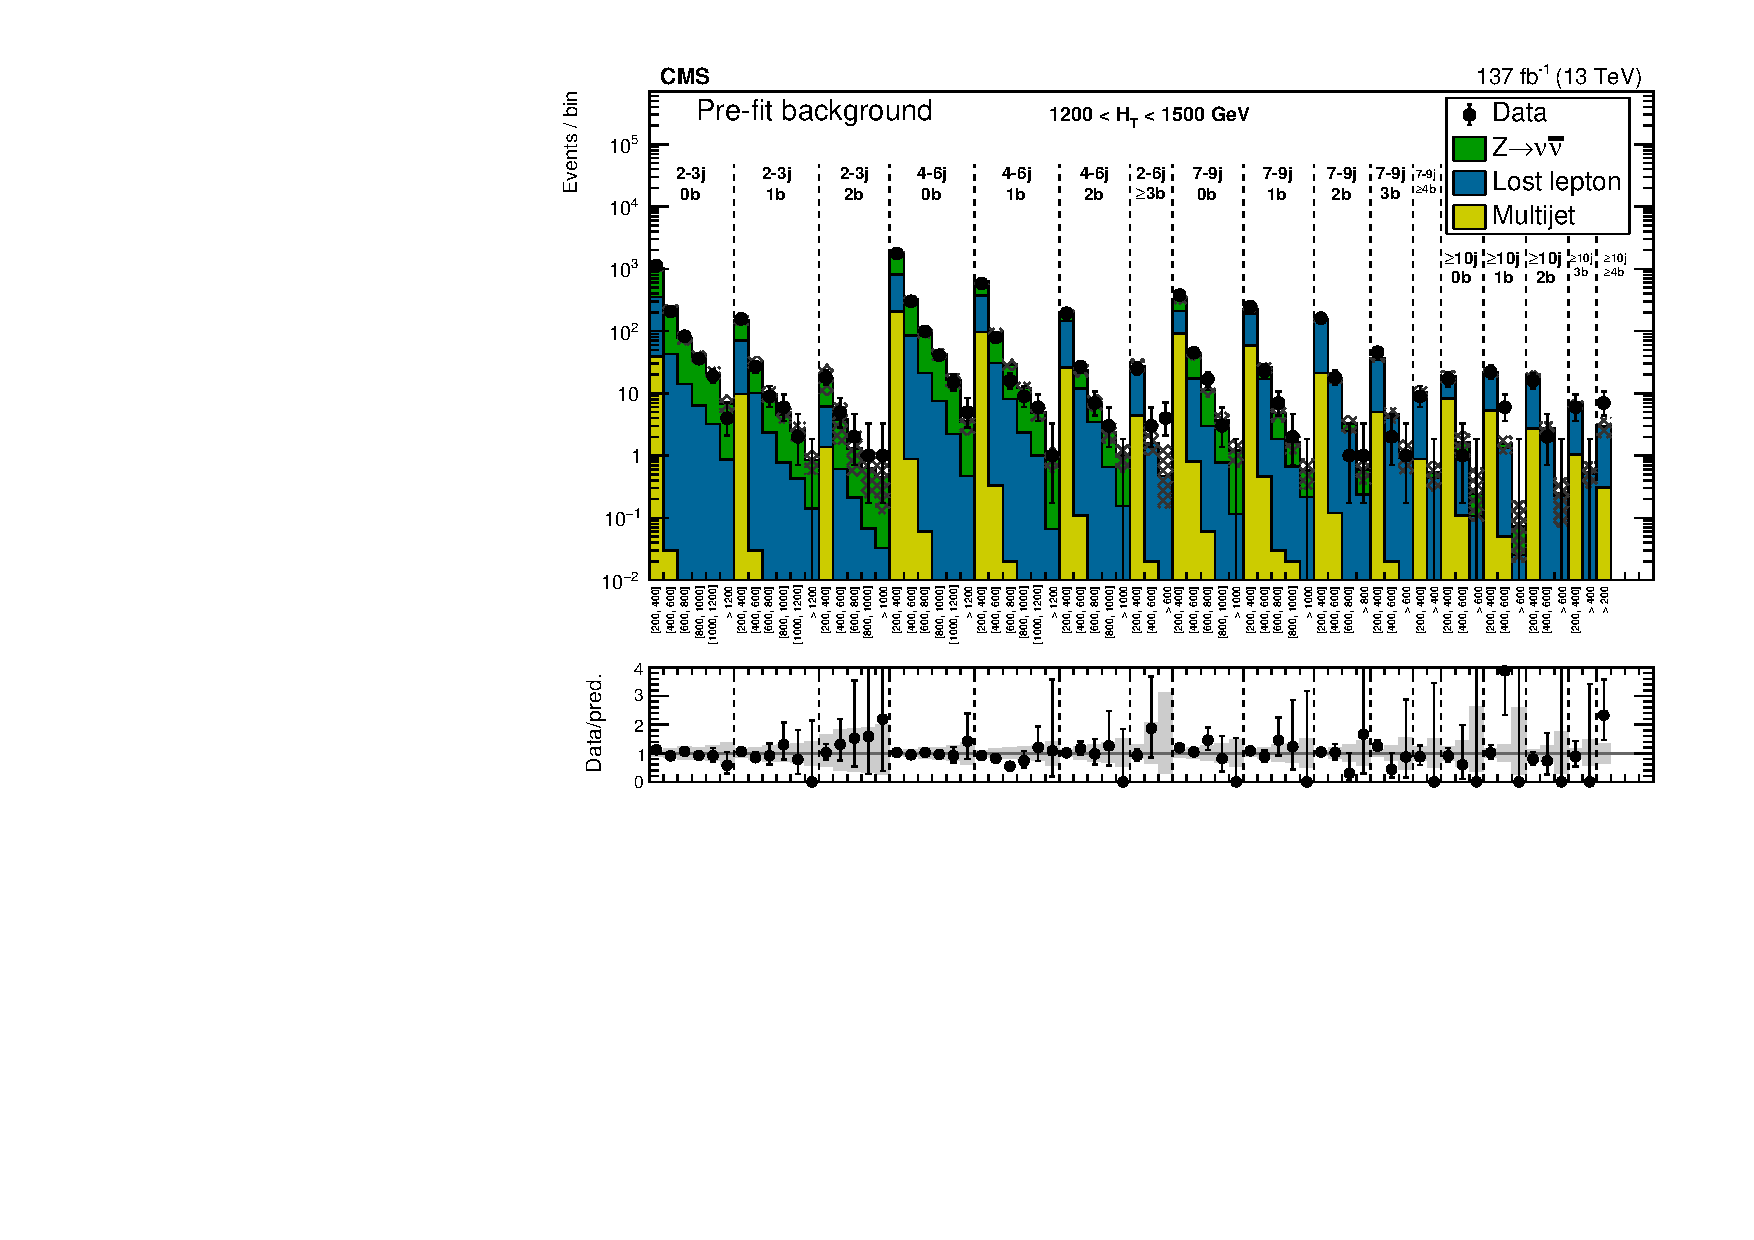
\includegraphics[width=0.93\textwidth]{figs/results/prefit_HT1200to1500_ratio.pdf} \\
    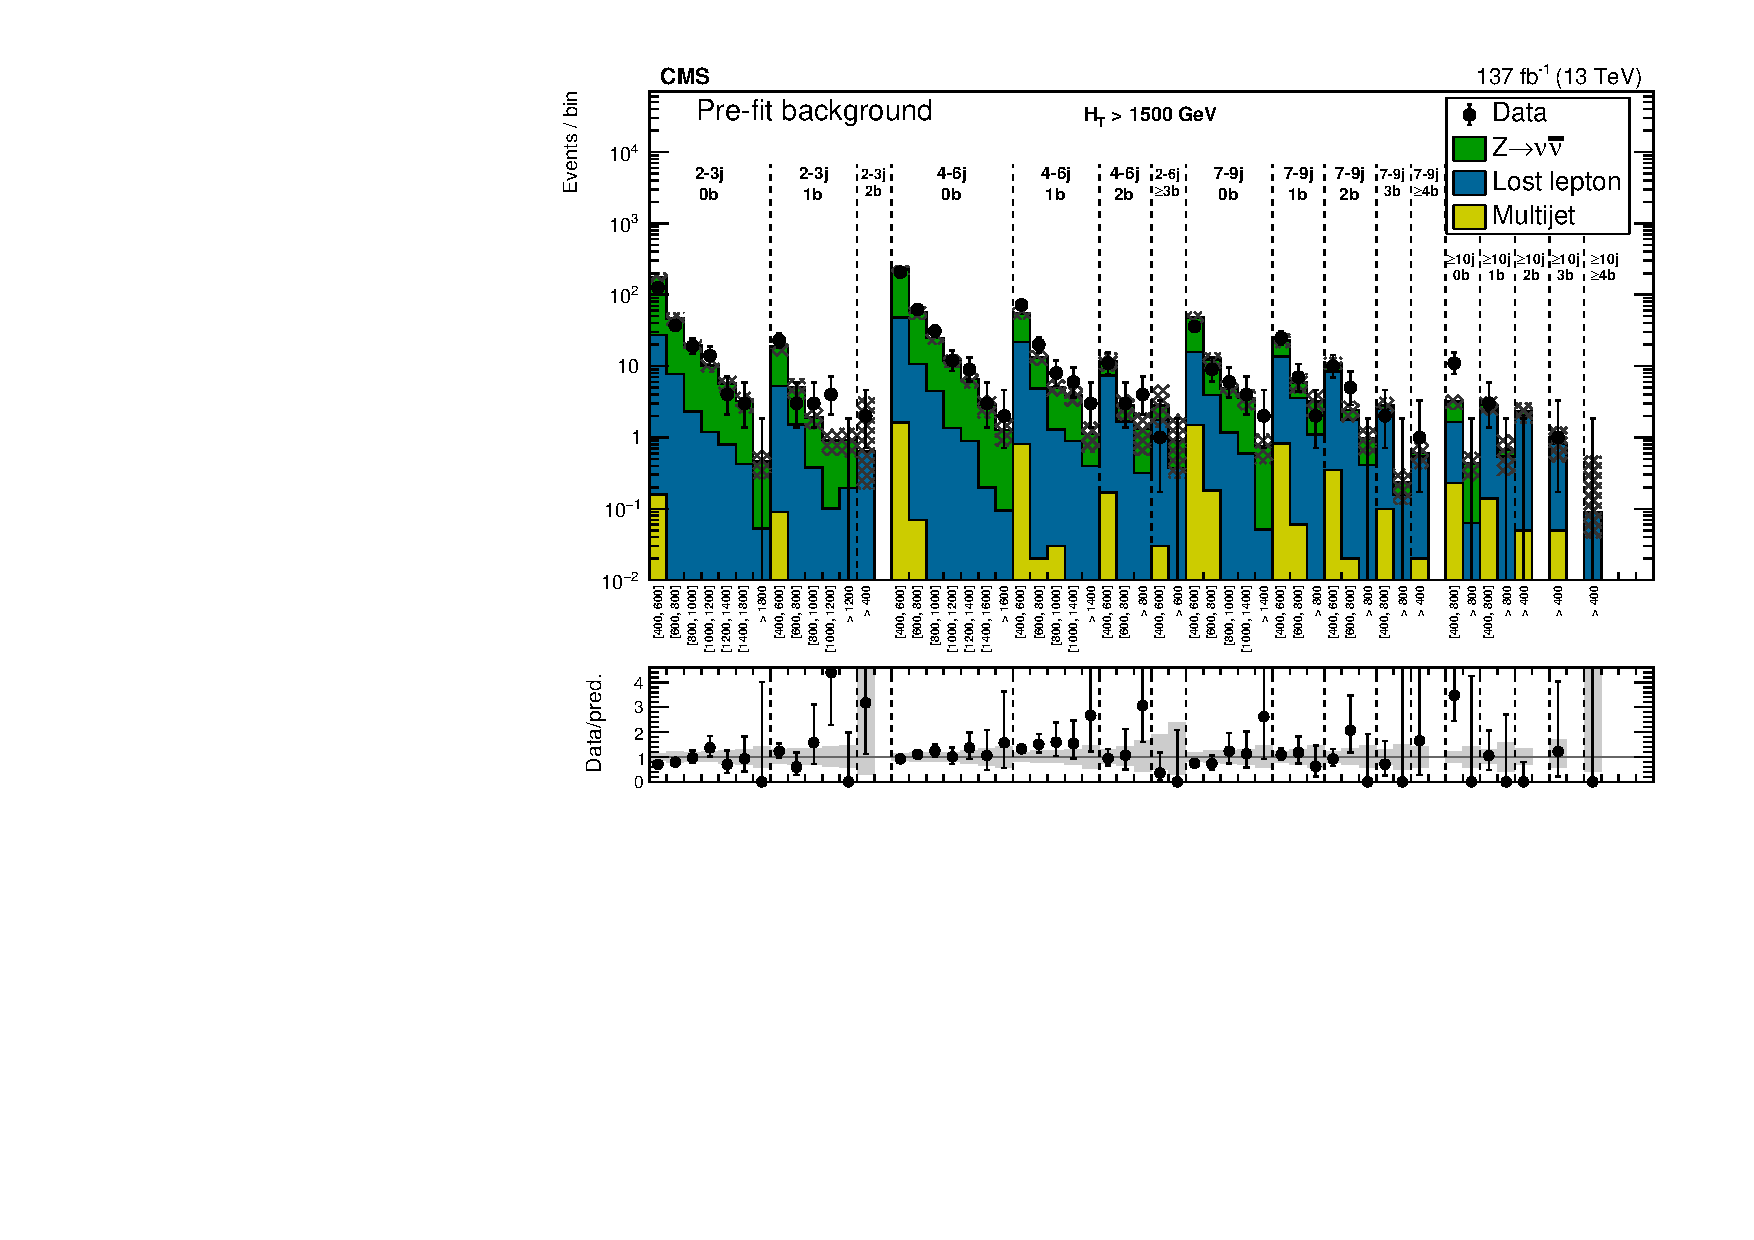
\includegraphics[width=0.93\textwidth]{figs/results/prefit_HT1500toInf_ratio.pdf} \\
    \caption{Expected (pre-fit) and observed yields for the full data set collected from
      2016--18, corresponding to an integrated luminosity of \Lint. The top and bottom figures
      contain the $\Nj\geq2$ signal regions for the $1200 \leq \Ht < 1500\GeV$ and $\Ht\geq1500\GeV$
      regions, respectively. \mttwo binning is shown on the $x$ axis, with the dashed lines separating
      bins by topological region.
            }
    \label{fig:results_h_uh}
  \end{center}
\end{figure}

\begin{figure}[htbp]
  \begin{center}
    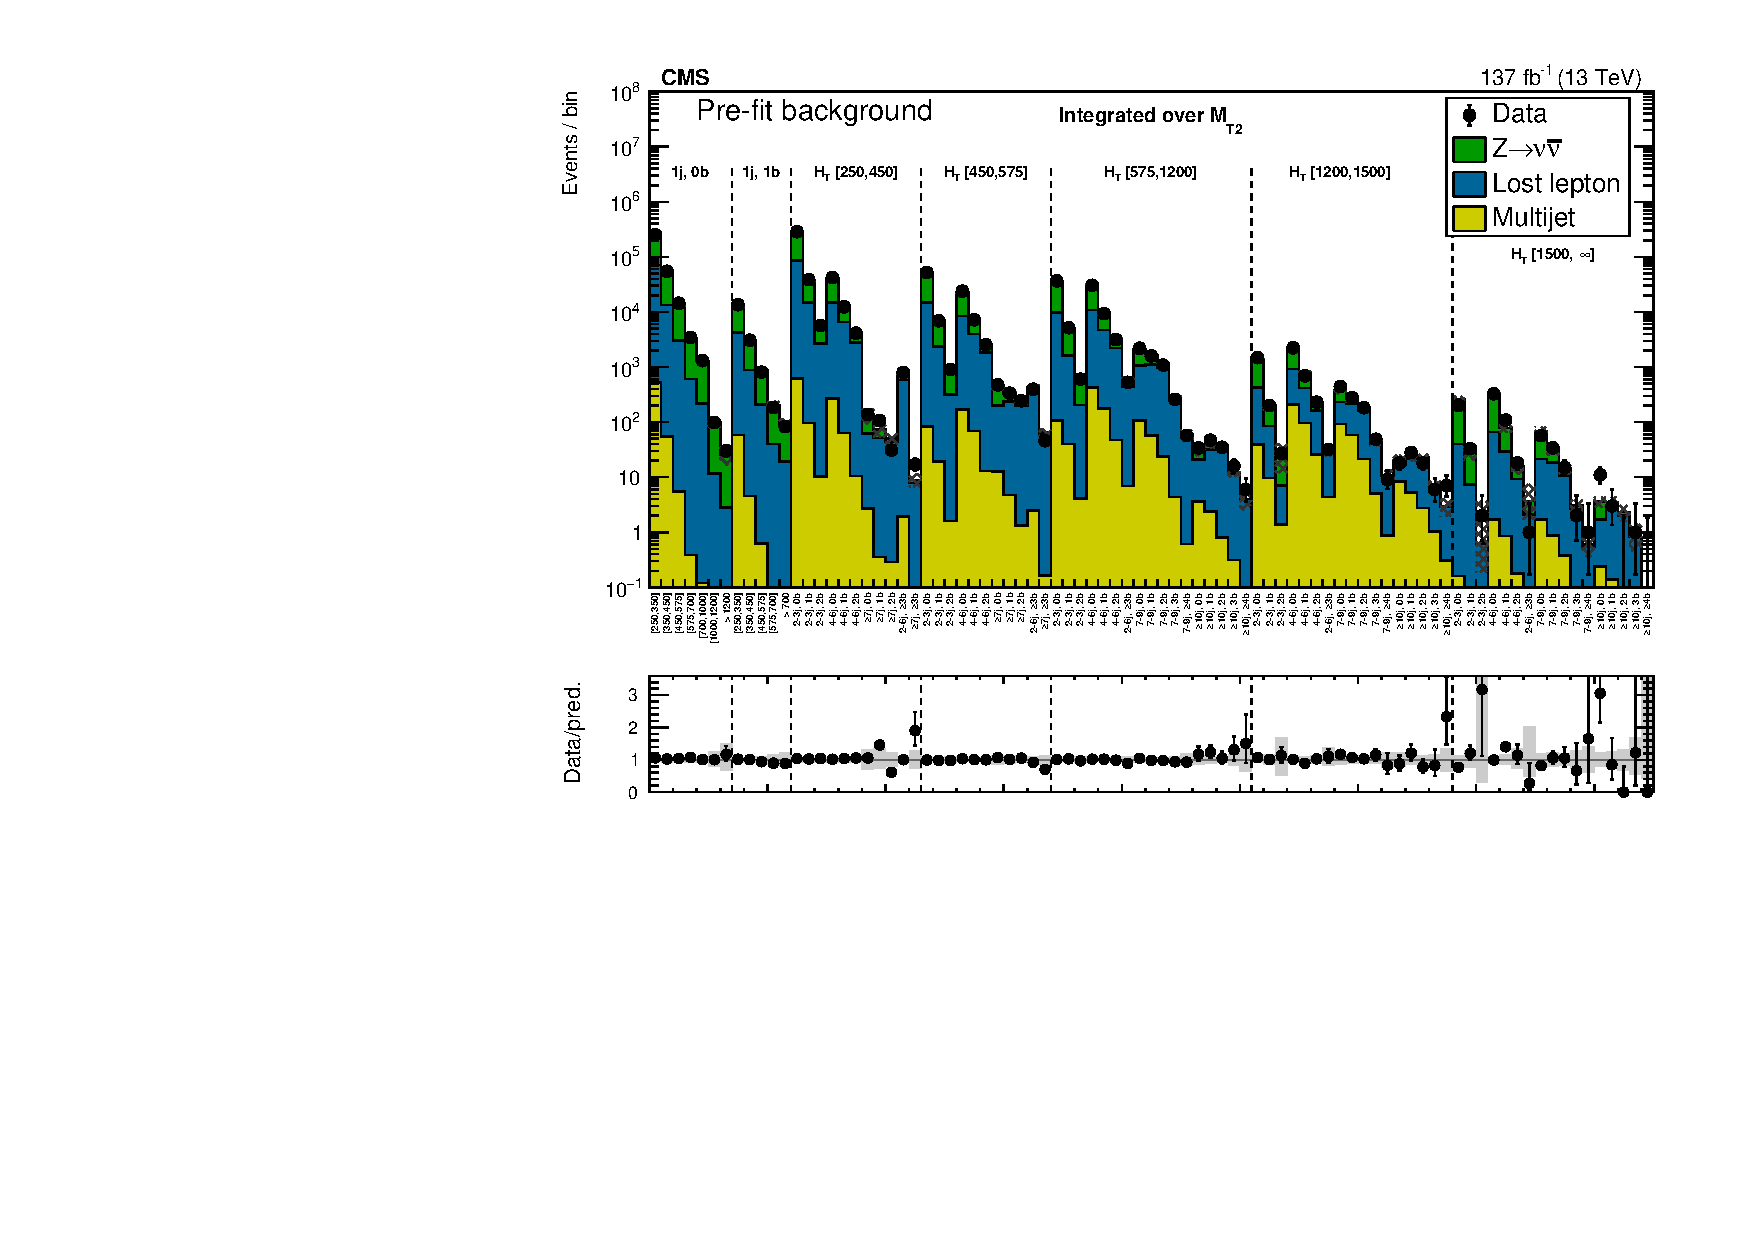
\includegraphics[width=0.93\textwidth]{figs/results/prefit_inclusive.pdf}
    \caption{Expected (pre-fit) and observed yields for the full data set collected from
      2016--18, corresponding to an integrated luminosity of \Lint. Here the results are shown
      integrated over \mttwo, with each bin on the $x$ axis corresponding to an \Nj/\Nb topological
      region. Dashed lines separate the various \Ht regions. The two leftmost regions contain the monojet
      signal regions, where the $x$ axis binning is $\pt^\mrm{jet1}$.
            }
    \label{fig:results_incl}
  \end{center}
\end{figure}


\section{Maximum-likelihood fits and the \texorpdfstring{CL$_\text{S}$}{CLs} technique}
\label{sec:fits}

The results presented in the previous section are \textit{pre-fit}, meaning the shown backgrounds
and uncertainties are straight from the estimation methods, without attempting to fit to the data
in any way. For the purposes of evaluating the results and setting constraints on models of new physics,
we apply a fitting procedure to test the compatibility of the observed results with SM predictions.

The expected background and signal yields are functions of \textit{nuisance parameters}, which control
the potential variations from all of the experimental and theoretical uncertainties. In practice these
are modeled as log-normal constraints on the background and signal yields (except for statistical uncertainties
on the observed control region event counts, which are modeled as gamma functions). Denoting the vector
of all nuisance parameters as $\boldsymbol\theta$, and their joint probability distribution as $p(\boldsymbol\theta)$, we can write
the complete likelihood function as
\be\label{eq:likelihood}
\mathcal{L}(\mrm{data}|\mu,\boldsymbol\theta) = \prod_{j\in\mrm{bins}} \frac{[\mu s_j(\boldsymbol\theta)+b_j(\boldsymbol\theta)]^{n_j}}{n_j!}
e^{-[\mu s_j(\boldsymbol\theta)+b_j(\boldsymbol\theta)]} p(\boldsymbol\theta),
\ee
where $s_j(\boldsymbol\theta)$ and $b_j(\boldsymbol\theta)$ are the predicted signal and background yields 
in bin $j$ (and which are functions of the nuisance parameters), $n_j$ is the observed event count in bin 
$j$, and $\mu$ is the signal strength parameter that we seek to set a constraint on. The likelihood is 
simply a product of Poisson probability terms with expectation $\mu s_j+b_j$ and observation $n_j$, and the 
PDF of the nuisance parameters, which is itself a product of log-normal and gamma functions.

To evaluate how well the estimated background fits the observed data, we could simply maximize this 
likelihood under the background-only hypothesis (i.e., set $\mu=0$ in Eq.~\ref{eq:likelihood}.
However, we would like to interpret this in the context of particular signal models, so we need a method
to evaluate the significance of the signal+background (S+B) assumption (the \textit{alternative hypothesis})
with respect to the background-only (B-only) assumption (the \textit{null hypothesis}).

To do this, we make use of the CL$_\mrm{S}$ technique~\cite{Read:CLs}.
First, a test statistic is defined as
\be
q_\mu = -2\log\frac{\mathcal{L}(\mu, \hat{\boldsymbol\theta}_\mu)}{\mathcal{L}(0, \hat{\boldsymbol\theta}_0)},
\ee
where the likelihood $\mathcal{L}$ is as defined in Eq.~\ref{eq:likelihood}, $\hat{\boldsymbol\theta}_0$
is the value of $\boldsymbol\theta$ that maximizes $\mathcal{L}$ for $\mu=0$, and $\hat{\boldsymbol\theta}_\mu$ is
the value of $\boldsymbol\theta$ that maximizes $\mathcal{L}$ for the given $\mu$. This is known as a
\textit{profile likelihood}, as we have profiled away the dependence on the nuisance parameters $\boldsymbol\theta$
by maximizing over them. Note that the denominator is independent of $\mu$, and is only there as a normalization.

We can construct distributions of $q_\mu$ for a given $\mu$ by generating random data, either under the B-only
or $\mu$S+B hypotheses. The values of $q_\mu$ under the $\mu$S+B hypothesis tend to be lower on average than those 
under the B-only hypothesis, as the numerator will be larger than the denominator (see top right plot in 
Fig.~\ref{fig:results_cls} for an example). The distributions converge as $\mu\to0$.

Using the actual observed data counts, we can then calculate the observed $q_\mu^\text{obs}$ for arbitrary $\mu$.
We then define
\be
\text{CL}_\text{S}(\mu) \equiv \frac{\text{CL}_\text{S+B}}{\text{CL}_\text{B}} \equiv
\frac{p(q_\mu\geq q_\mu^\text{obs}\;|\;\mu\text{S+B})}{p(q_\mu\geq q_\mu^\text{obs}\;|\;\text{B})}
\ee

Note that $\text{CL}_\text{S}(\mu)$ is exactly equal to 1 at $\mu=0$, and is a strictly decreasing function of $\mu$.
One can think of $\text{CL}_\text{S}$ as the relative likelihood that the observed counts would look as ``background-like''
as they do under the $\mu$S+B hypothesis versus the B-only hypothesis. When CL$_\text{S}$ is very small,
we can be pretty confident that the $\mu$S+B assumption is \textit{not} supported by the data. Thus, we define
an upper limit on $\mu$ at the $1-\alpha$ confidence level as the $\mu_{1-\alpha}$ that satisfies
\be
\text{CL}_\text{S}(\mu_{1-\alpha}) = \alpha
\ee

This process is illustrated in Fig.~\ref{fig:results_cls} for a toy experiment with 3 bins. We predict event counts of 
10, 5, and 2, with an uncorrelated 20\% uncertainty on each. Nominal expected signal with $\mu=1$ is
2 events in each bin. We observe event counts of 7, 6, and 1. The top left panel shows the expected and observed
yields in each bin. The top right panel shows distributions of $q_{\mu=1}$ under the B and S+B hypotheses, the
observed value of $q_{\mu=1}^\text{obs}=3.75$, and shaded areas representing CL$_\text{S+B}$ and $1-\text{CL}_\text{B}$
The bottom panel shows CL$_\text{S}(\mu)$ as a function of $\mu$, and the 95\% confidence level upper limit
on $\mu$ of 1.14, computed by finding the $\mu$ value at which CL$_\text{S}(\mu)$ crosses below 0.05.

\begin{figure}[htbp]
  \begin{center}
    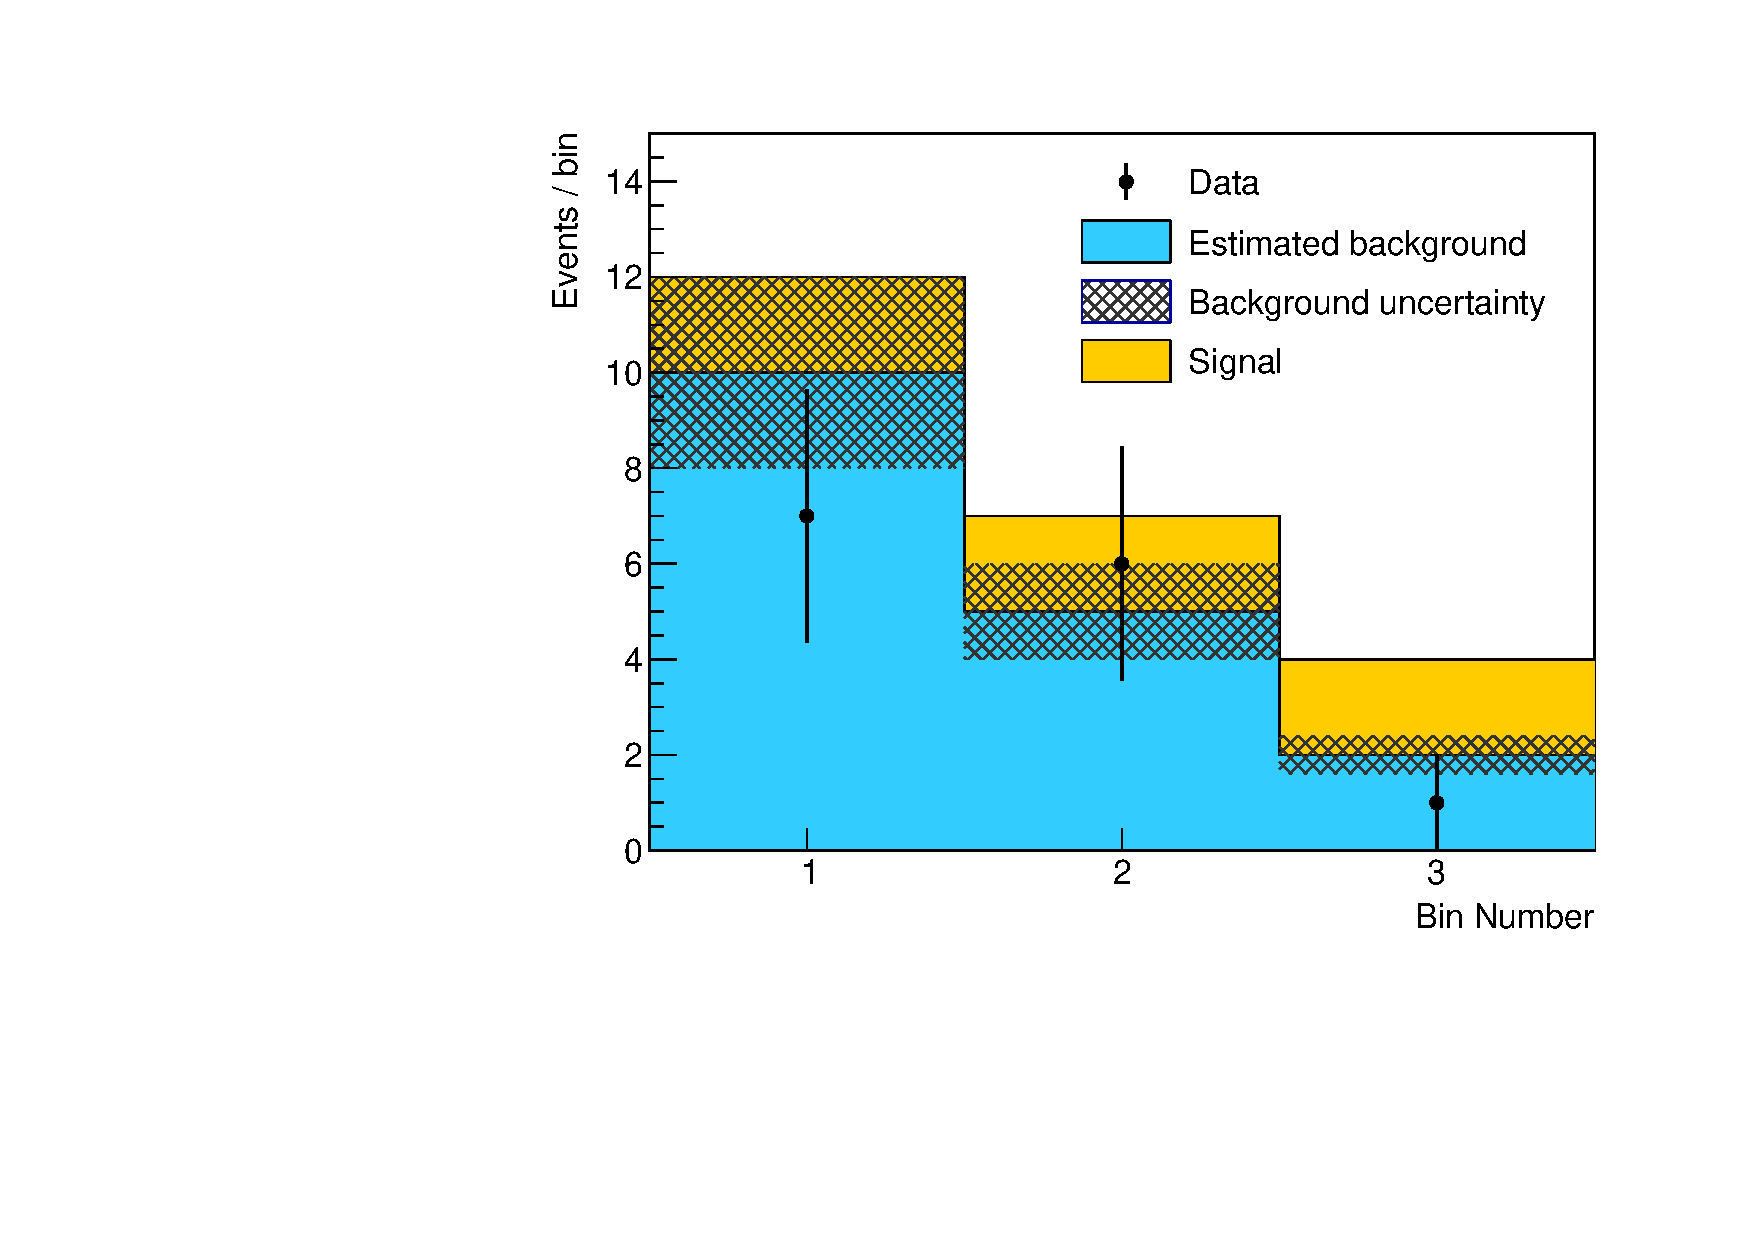
\includegraphics[width=0.48\textwidth]{figs/results/toy_exp.pdf}
    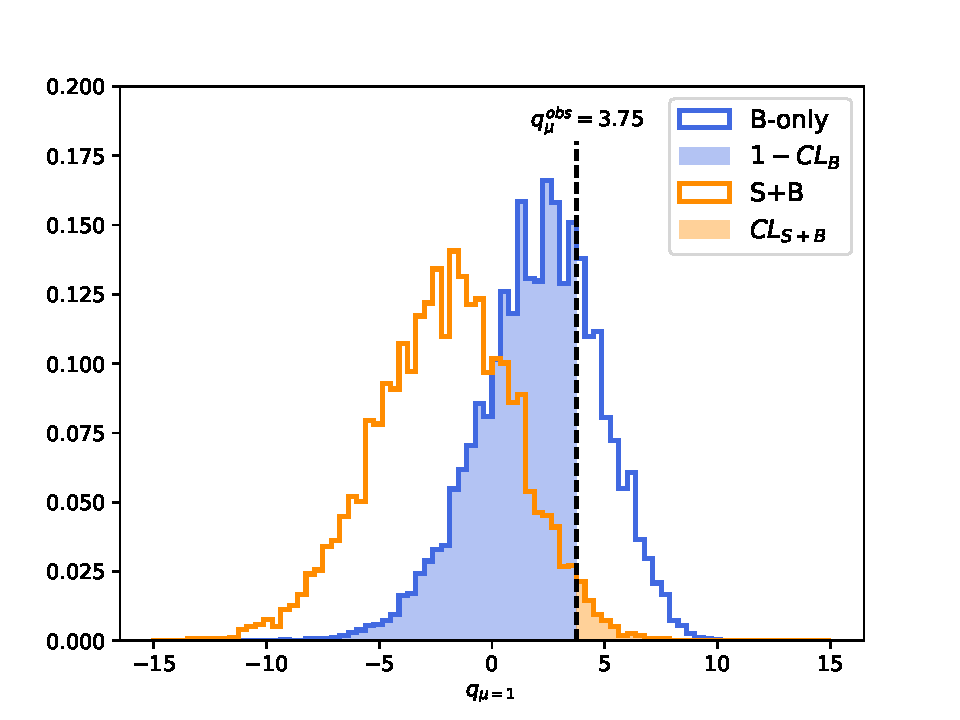
\includegraphics[width=0.48\textwidth]{figs/results/qmu_dist.pdf} \\
    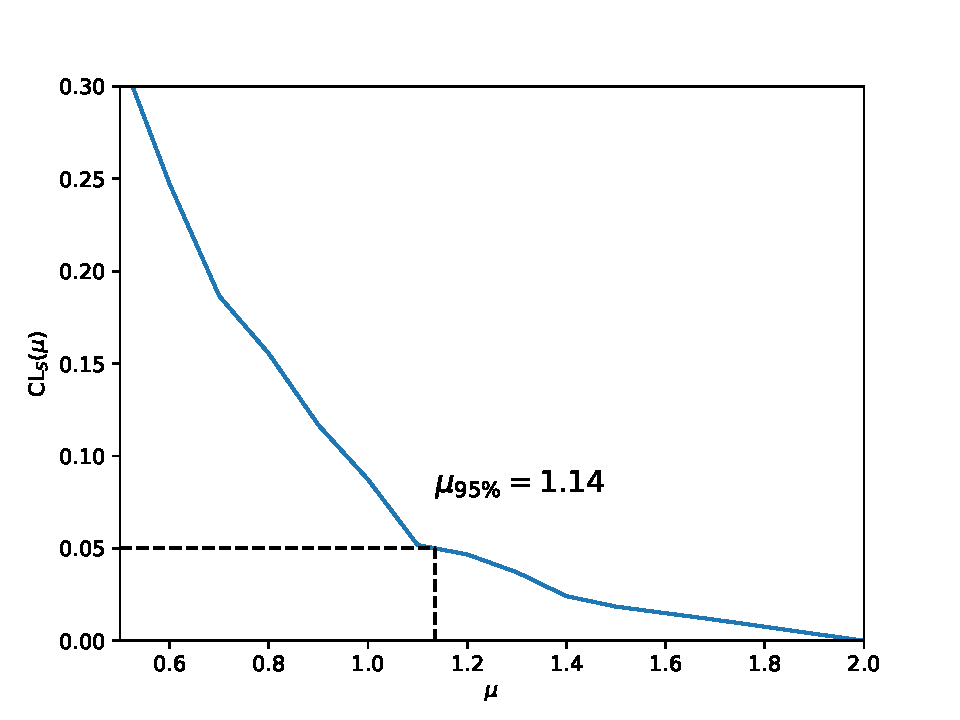
\includegraphics[width=0.48\textwidth]{figs/results/cls.pdf}
    \caption{An example calculation of an upper limit on signal strength $\mu$ with a three-bin toy experiment.
      The estimated background, background uncertainty, and signal yields, as well as the observed counts, are shown
      in the top left. On the top right, distributions of $q_{\mu=1}$ are shown for both the B-only and S+B
      hypotheses. The dotted line shows the observed value of $q_{\mu=1}^\text{obs}=3.75$, and the blue and orange
      shaded areas represent $1-\text{CL}_\text{B}$ and $\text{CL}_\text{S+B}$, respectively. The bottom plot
      shows CL$_\text{S}(\mu)=\text{CL}_\text{S+B}/\text{CL}_\text{B}$ as a function of $\mu$, and the observed
      95\% confidence level upper limit on $\mu$ of 1.14, found by locating the point where CL$_\text{S}$
      crosses below $1-0.95=0.05$.
            }
    \label{fig:results_cls}
  \end{center}
\end{figure}

The $\text{CL}_\text{S}$ method outlined above is used to set limits on all of the signal models in the following
sections. Due to the very large number of bins in the \mttwo analysis, it is computationally infeasible
to compute distributions of the test statistic explicitly. Hence, we use an \textit{asymptotic approximation} to
derive the distributions necessary to calculate $\text{CL}_\text{S}$, as described in~\cite{Cowan:asymptotic}.
This has been verified at a smaller number of signal points to give results consistent with the exact method.
The calculations are performed with a CMS-produced wrapper around RooFit~\cite{roofit}.

\section{Interpretations}
\label{sec:interp}

The statistical procedure described in the previous section is used to set 95\% confidence level upper limits
on the cross sections of a variety of signal models. 
For the interpretation of the results, simplified BSM physics models~\cite{Alwall:sms,Alwall:jetmet,Alves:sms} are used. 
Simplified models are defined by sets of hypothetical particles and sequences of their production
and decay. The theoretical parameters are thus reduced to a small number of masses and cross
sections, providing an effective tool to characterize potential signals of BSM physics.

The estimation of the three different background types
and the corresponding uncertainties are described in Chapters~\ref{chap:zinv} through \ref{chap:qcd}.
Estimated signal yields are taken from simulation, which has been produced using the CMS fast simulation
framework~\cite{CMS:fastsim}. Due to known mis-modeling of ISR jets in simulation, signal samples
have been re-weighted based on the number of generator-level ISR jets, with weights derived from a
\ttbar-enriched sample in data. In addition, due to known \ptmiss tail mis-modeling in the fast simulation,
estimated signal yields are computed using an average of the generator-level and reconstructed \ptmiss
values. Systematic uncertainties to account for both of these procedures are applied to the estimated
signal yields in each bin.

A list of all sources of uncertainty on the signal yields is given in Table~\ref{tab:sig_systs}, along
with the range of values for each uncertainty source over all analysis bins.

\begin{table}[htb]
\caption{
Systematic uncertainties in the signal yields for the simplified models of BSM physics.
The large statistical uncertainties in the simulated signal sample come from a small number of bins with low acceptance,
which are typically not among the most sensitive bins contributing to a given model benchmark point.
    \label{tab:sig_systs}}
\centering
\begin{tabular}{lc}
\hline
Source & Range [\%] \\
\hline
Integrated luminosity                     & 2.3--2.5     \\
Limited size of MC samples                & 1--100  \\
Renormalization and factorization scales  & 5       \\
ISR modeling                              & 0--30   \\
b tagging efficiency, heavy flavors       & 0--40   \\
b tagging efficiency, light flavors       & 0--20   \\
Lepton efficiency                         & 0--20   \\
Jet energy scale                          & 5       \\
Fast simulation \ptmiss\ modeling            & 0--5     \\
\hline
\end{tabular}
\end{table}

\subsection {Supersymmetry models}

A total of 11 $R$-parity conserving supersymmetry simplified models are considered, illustrated
in Fig.~\ref{fig:SMS_susy}.
For each scenario of gluino (squark) pair production, the simplified models assume that
all SUSY particles other than 
those shown in the corresponding diagram
are too heavy to be produced directly, and that the gluino (squark) decays promptly.
The models assume that each gluino (squark) decays with a 100\% branching fraction 
into the decay products depicted in Fig.~\ref{fig:SMS_susy}.
For models where the decays of the two gluinos or squarks in the same diagram differ, a 1/3 (1/2)
branching fraction for each of the three (two) decay modes is assumed.
In particular, for the diagram of gluino pair production where the decays of the two gluinos 
differ, each gluino can decay via a \chizz, \charginoplus, or \charginominus.
For scenarios with top squarks decaying into top quarks, the polarization of the
top quark can be model dependent and a function of the top squark and neutralino mixing matrices.
To maintain independence of any particular model realization, 
events are generated with unpolarized top quarks.
Signal cross sections are calculated at approximately NNLO+NNLL (next-to-next-to-leading-logarithm) order in 
$\alpha_{\mathrm{s}}$~\cite{Beenakker:nnll}.
For direct light-flavor squark pair production we assume either one single squark, 
or eight degenerate squarks ($\SQqL+\SQqR$, with $\SQq=\SQu,\;\SQd,\;\SQs,\;\text{or}\;\SQc$). 
For direct bottom and top squark pair production, we assume one single squark.


\begin{figure}[htbp]
  \centering
    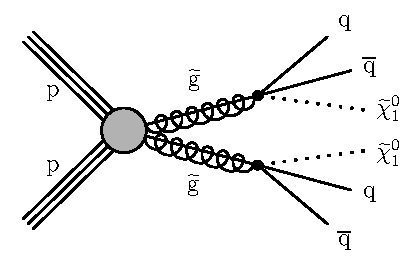
\includegraphics[width=0.3\textwidth]{figs/results/T1qqqq.pdf}
    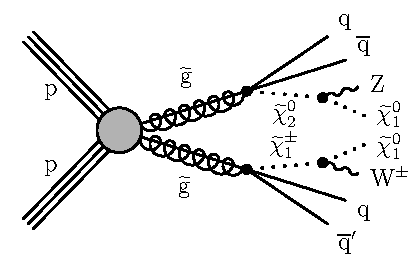
\includegraphics[width=0.3\textwidth]{figs/results/T5qqqqWZ.pdf}
    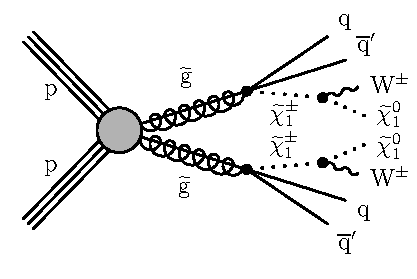
\includegraphics[width=0.3\textwidth]{figs/results/T5qqqqWW.pdf}\\
    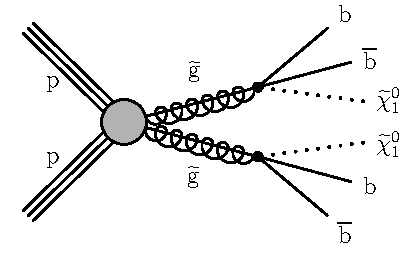
\includegraphics[width=0.3\textwidth]{figs/results/T1bbbb.pdf}
    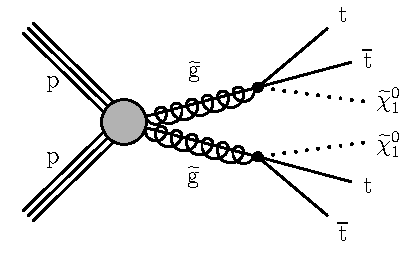
\includegraphics[width=0.3\textwidth]{figs/results/T1tttt.pdf} \\
    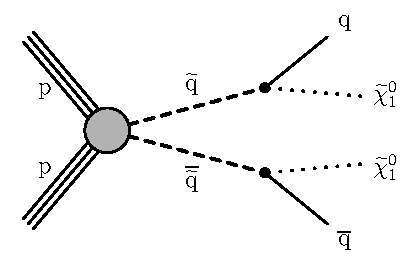
\includegraphics[width=0.3\textwidth]{figs/results/T2qq.pdf}
    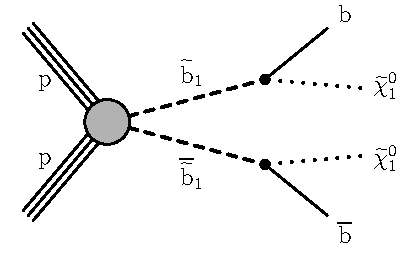
\includegraphics[width=0.3\textwidth]{figs/results/T2bb.pdf}
    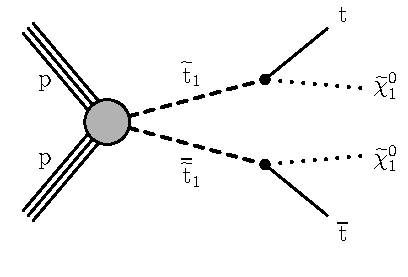
\includegraphics[width=0.3\textwidth]{figs/results/T2tt.pdf} \\
    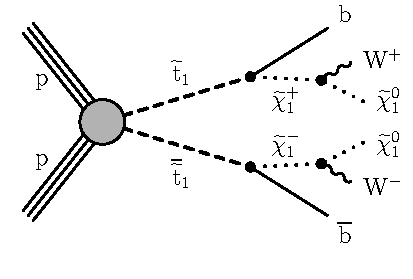
\includegraphics[width=0.3\textwidth]{figs/results/T2bW.pdf}
    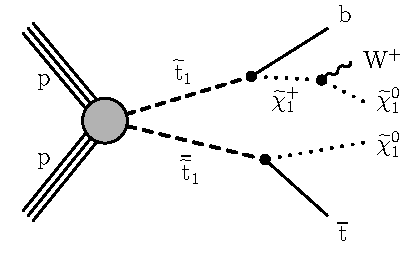
\includegraphics[width=0.3\textwidth]{figs/results/T2bt.pdf}
    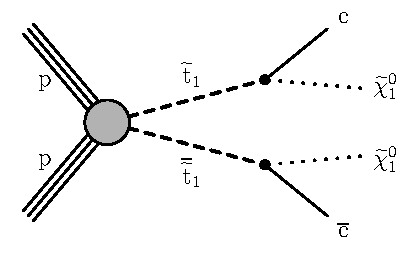
\includegraphics[width=0.3\textwidth]{figs/results/T2cc.pdf} \\
    \caption{(Upper) Diagrams for three scenarios of gluino-mediated light-flavor squark pair production with different decay modes.
    For mixed decay scenarios, we assume equal branching fraction for each decay mode.
    (Upper middle) Diagrams for the gluino-mediated bottom squark and top squark pair production.
      (Lower middle) Diagrams for the direct pair production of light-flavor, bottom and top squark pairs.
      (Lower) Diagrams for three alternate scenarios of direct top squark pair production with different decay modes.
      For mixed decay scenarios, we assume equal branching fraction for each decay mode.}
    \label{fig:SMS_susy}
\end{figure}

Figure~\ref{fig:t5x} shows the exclusion limits at 95\% CL for direct gluino pair production where the
gluinos decay to light-flavor quarks under three different decay scenarios. Exclusion limits for
direct gluino pair production where the gluinos decay to bottom and top quarks are shown in
Fig.~\ref{fig:t1x}, and those for the direct production of squark pairs are shown in Fig.~\ref{fig:t2x}. Three alternate
decay scenarios are also considered for the direct pair production of top squarks, and their
exclusion limits are shown in Fig.~\ref{fig:stop_other}.

Table~\ref{tab:lim_susy} summarizes the limits on the masses of SUSY particles excluded for the simplified
model scenarios considered. These results extend the constraints on gluino and squark masses
by about 100--350\GeV and on the \lsp mass by 100--250\GeV with respect to the limits
in the previous iteration of this analysis \cite{CMS:mt22016}.

\begin{table*}[htb]
  \caption{Summary of the observed 95\% CL exclusion limits on the masses of SUSY particles for different simplified model scenarios.
    The highest limits on the mass of the directly produced particles and on the mass of the \lsp are quoted.
    \label{tab:lim_susy}}
  \centering
  \begin{tabular}{lrr}
    \hline
    Simplified & Highest limit on directly produced  & Highest limit on \\
    model & SUSY particle mass [\GeV] & \lsp mass [\GeV] \\
    \hline\hline
    Direct gluino pair production: & & \\
    $\gluino\to \qqbar\lsp$ & 1970 & 1200 \\
    $\gluino \to \qqbar Z\lsp$ or $\gluino \to \qqbarpr W^\pm\lsp$ & 2020 & 1090 \\
    $\gluino\to b\bar{b}\lsp$ & 2250 & 1525 \\
    $\gluino\to \ttbar\lsp$ & 2250 & 1250 \\
    \hline
    Direct squark pair production: & & \\
    Eight degenerate light squarks & 1710 & 870 \\
    Single light squark & 1250 & 525 \\
    Bottom squark & 1240 & 700 \\
    Top squark & 1200 & 580 \\
    \hline
  \end{tabular}
\end{table*}

\begin{figure}[htbp]
  \centering
    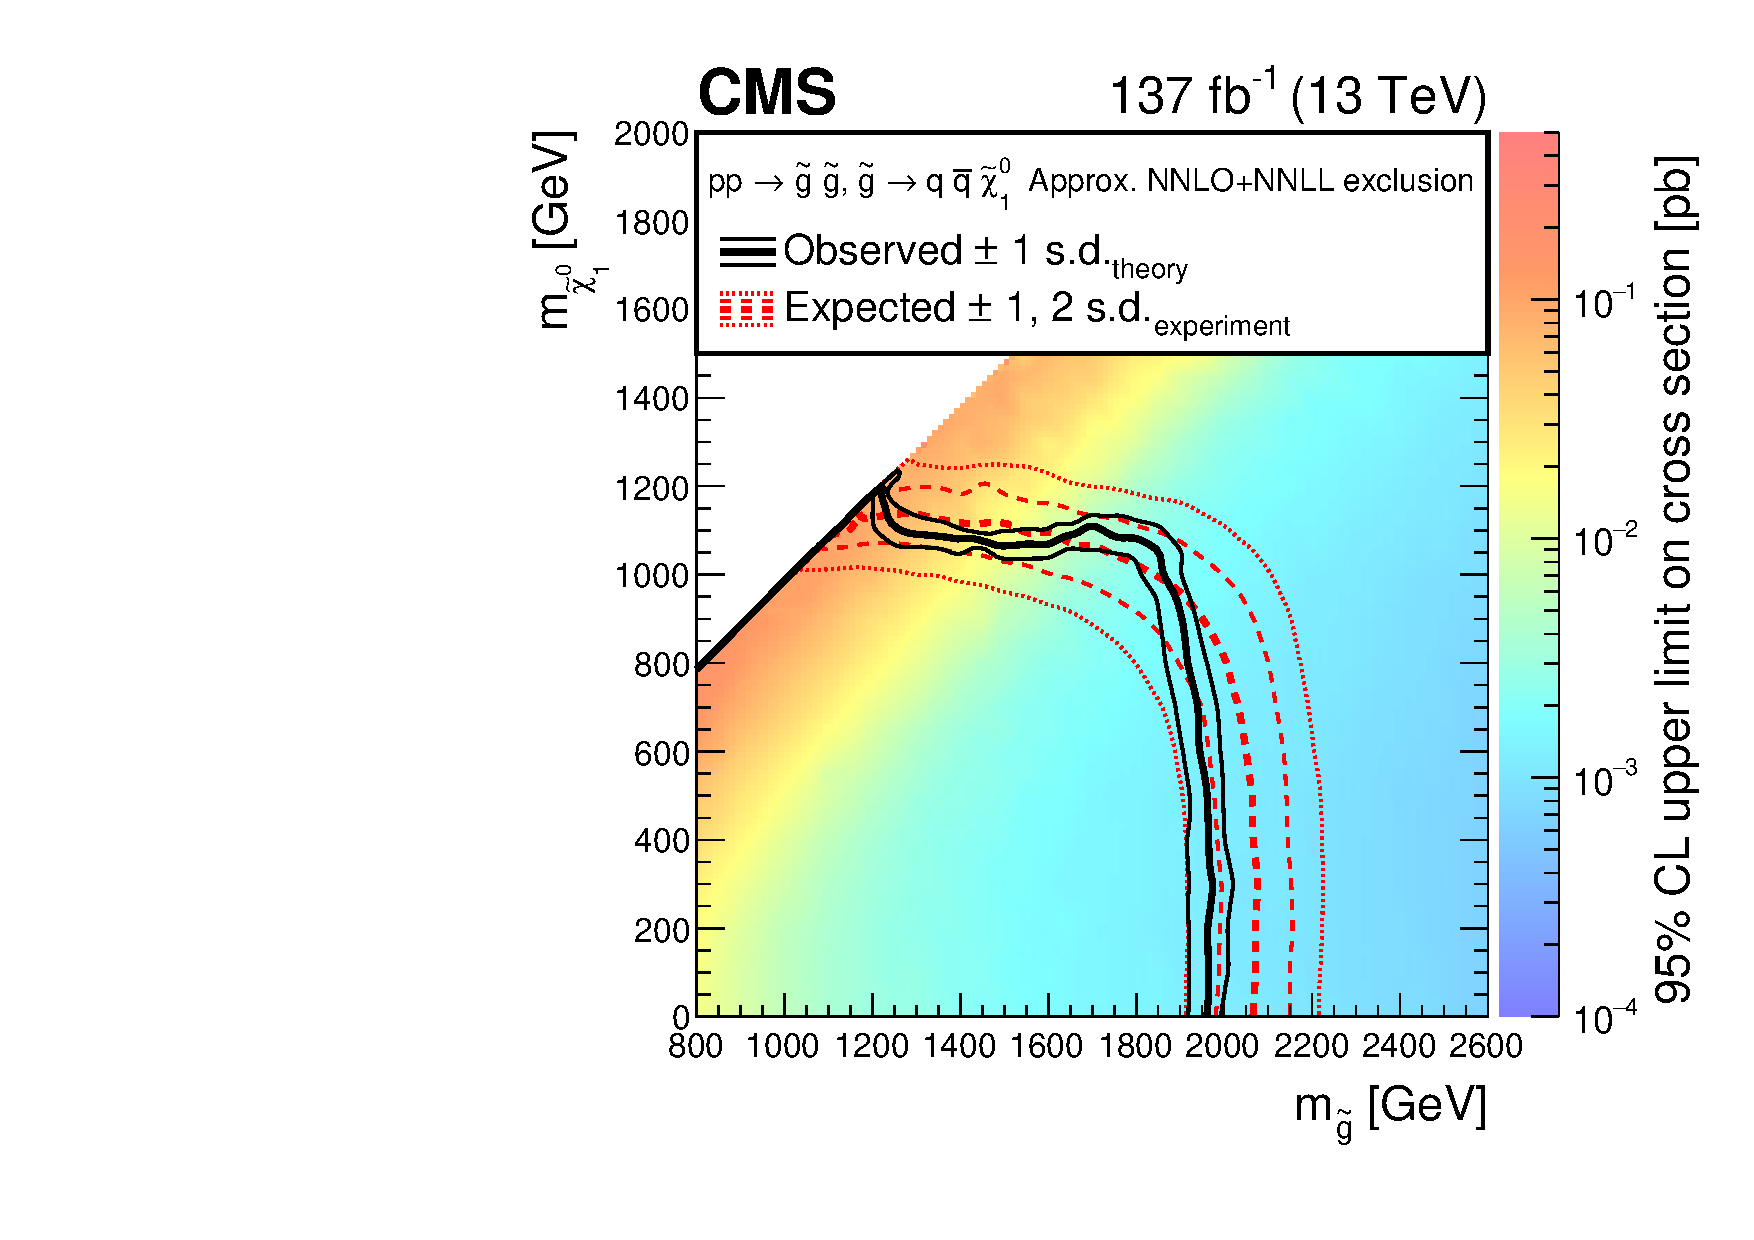
\includegraphics[width=0.48\textwidth]{figs/results/T1qqqqXSEC.pdf}\\
    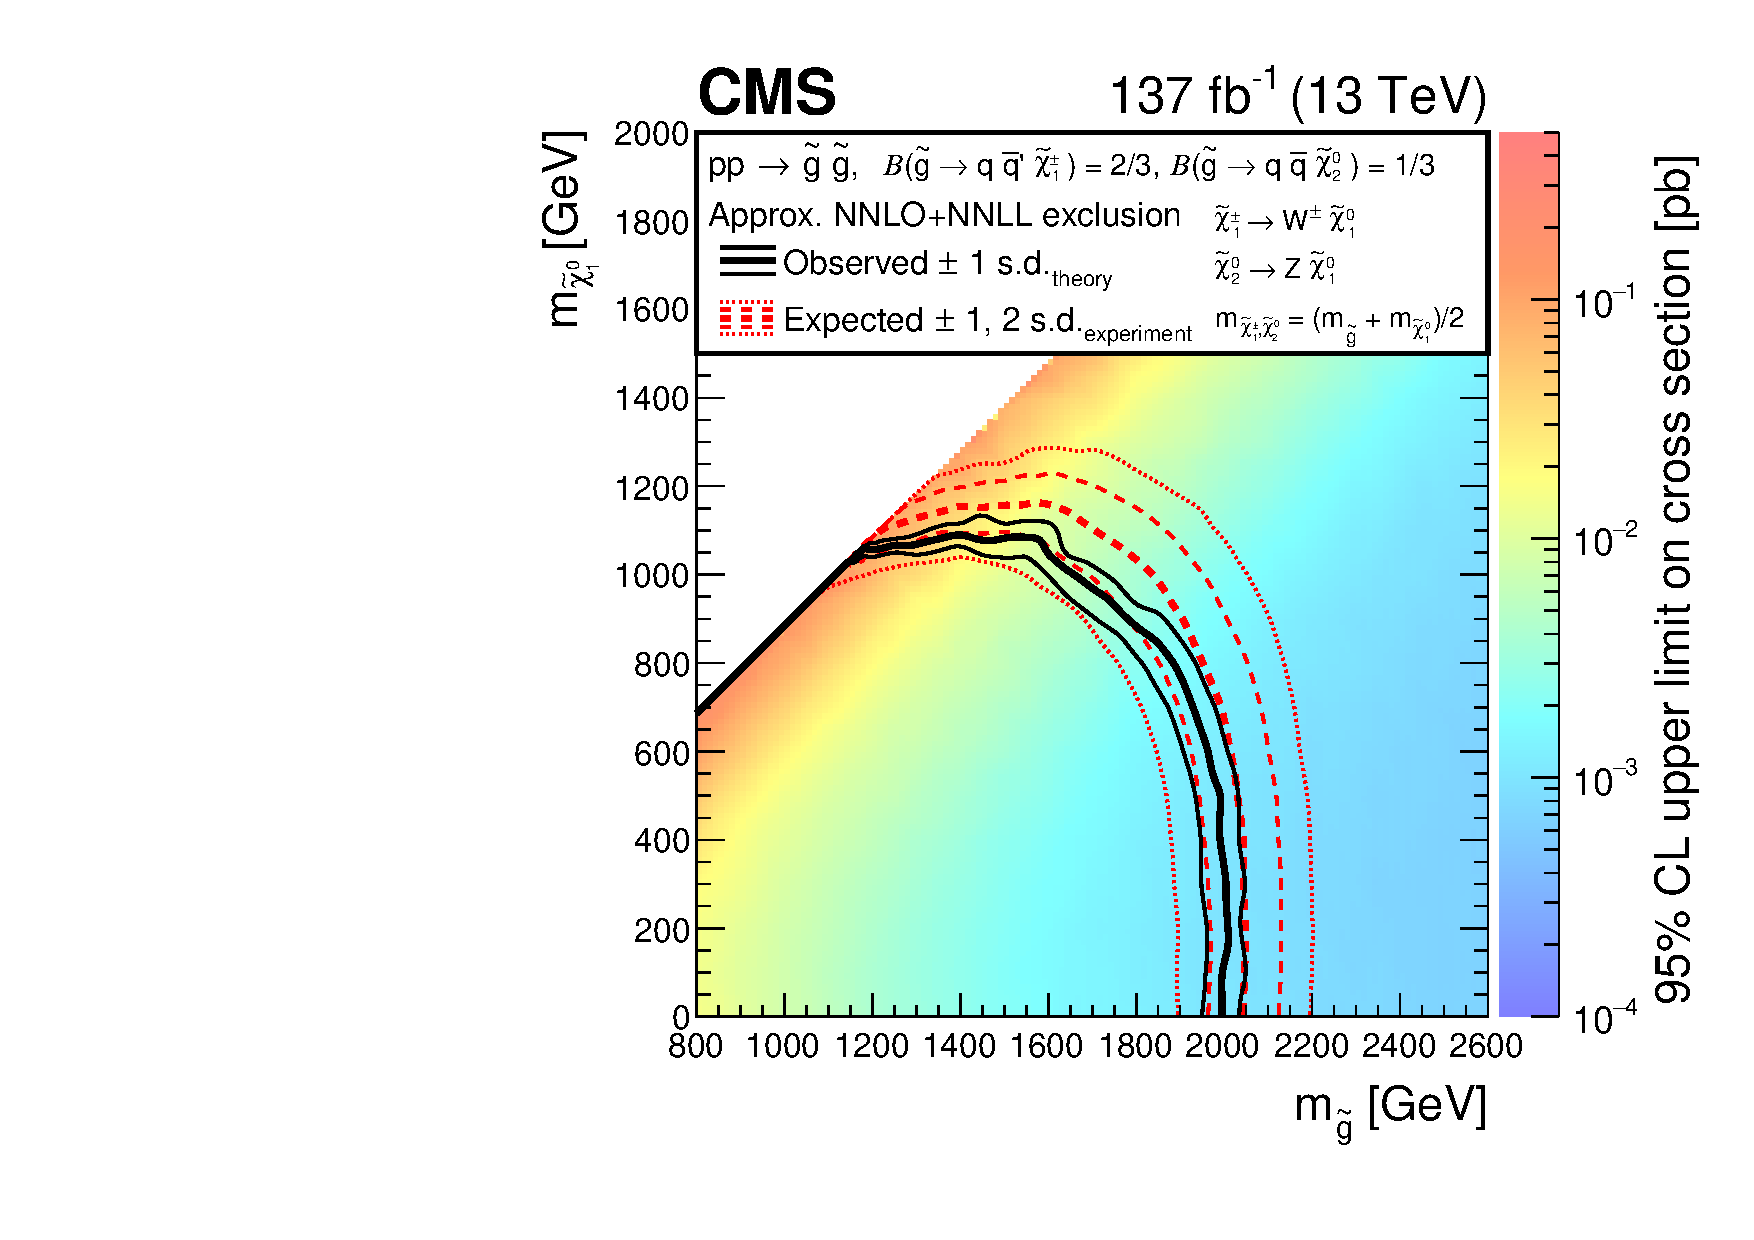
\includegraphics[width=0.48\textwidth]{figs/results/T5qqqqVVXSEC.pdf}
    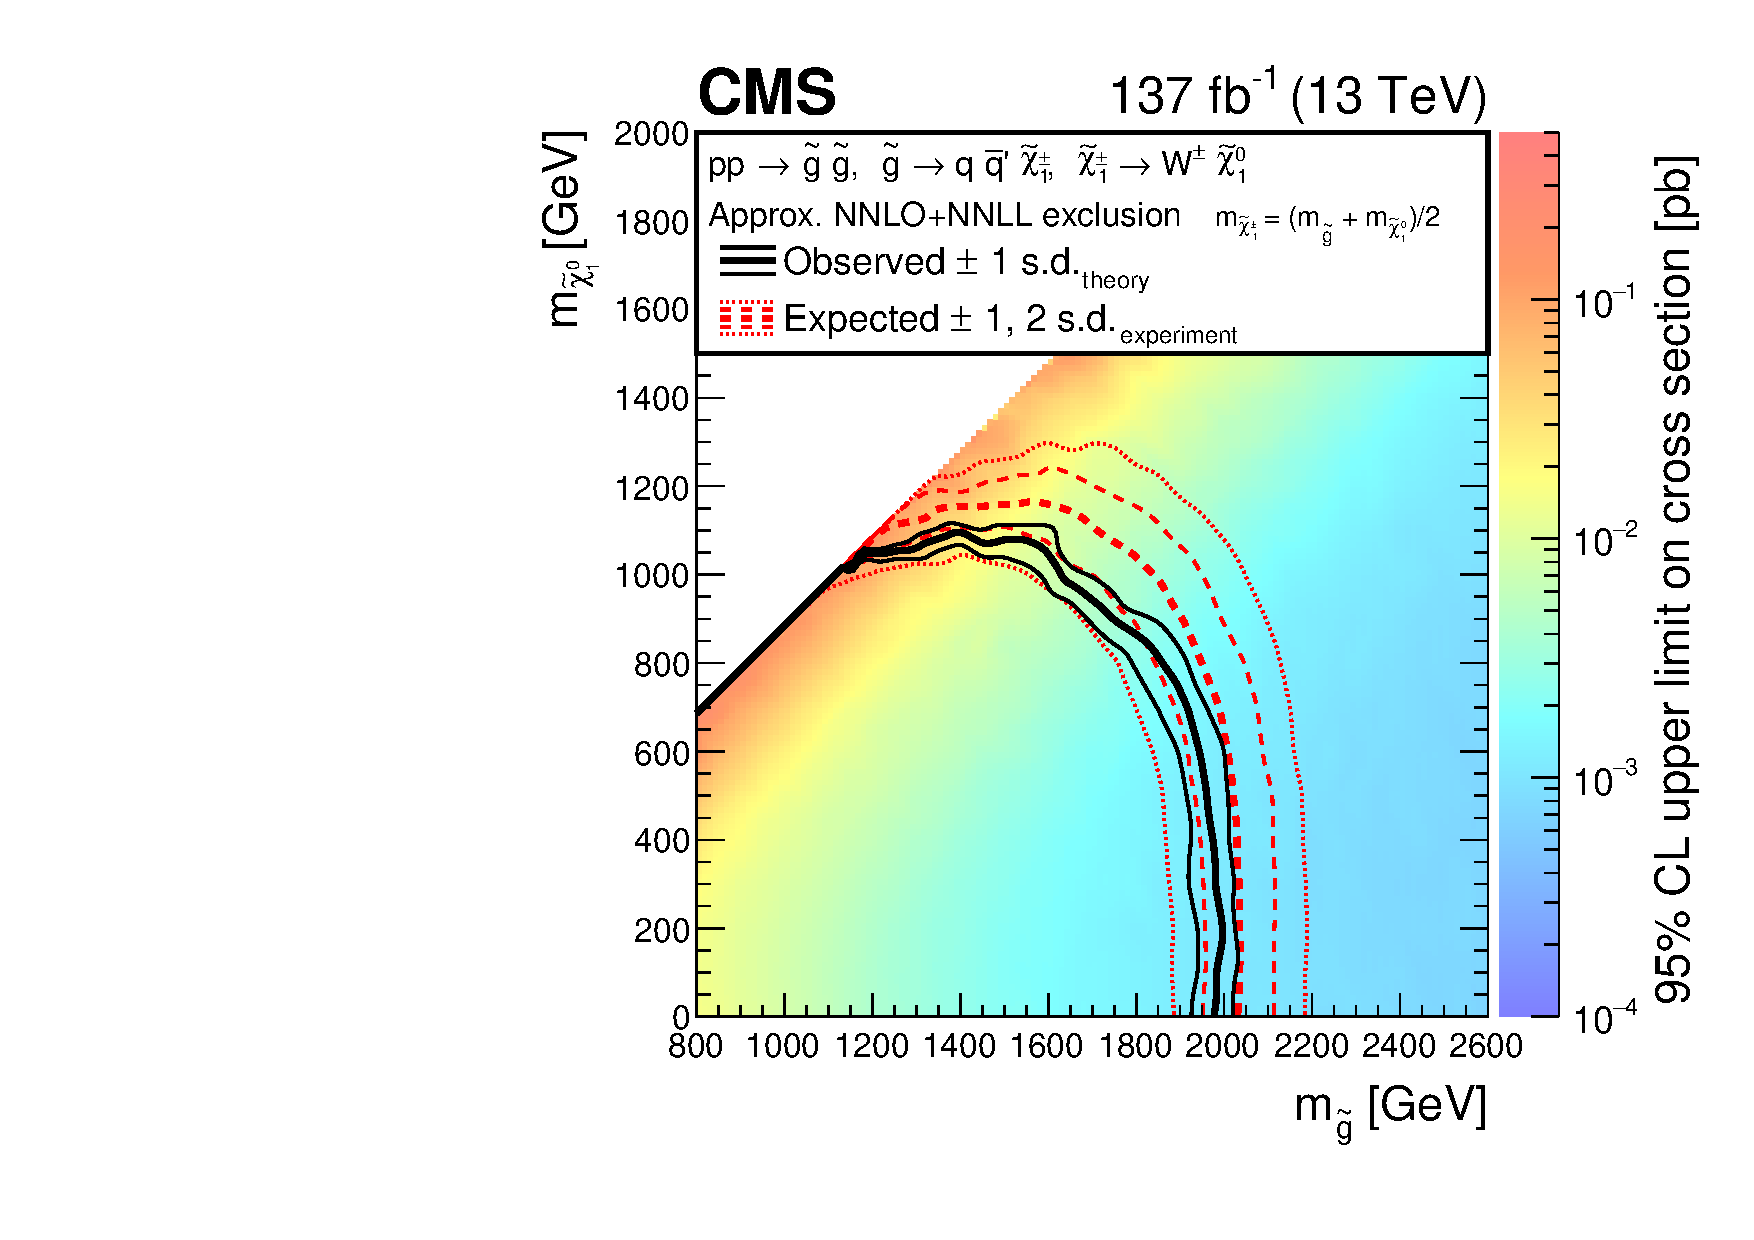
\includegraphics[width=0.48\textwidth]{figs/results/T5qqqqWWXSEC.pdf}
    \caption{
    Exclusion limits at  95\% CL for direct gluino pair production,
    where (upper) $\gluino \to \qqbar\lsp$, (lower left) $\gluino \to \qqbar\chizz~\mathrm{and}~\chizz \to Z\lsp$, or $\gluino \to \qqbarpr\chargino~\mathrm{and}~\chargino \to W^\pm\lsp$, and
    (lower right) $\gluino \to \qqbarpr\chargino~\mathrm{and}~\chargino \to W^\pm\lsp$ (with $q=u,\;d,\;s,\;\text{or}\;c$).
    For the scenarios where the gluinos decay via an intermediate \chizz or \chargino, \chizz and \chargino are assumed to be mass-degenerate, with
     $m_{\chargino,~\chizz}=0.5(m_{\gluino}+m_{\lsp})$.
      The area enclosed by the thick black curve represents the observed exclusion region,
      while the dashed red lines indicate the expected limits and
      their $\pm$1 and $\pm$2 standard deviation ranges.
      The thin black lines show the effect of the theoretical
      uncertainties in the signal cross section.
      Signal cross sections are calculated at approximately NNLO+NNLL order in $\alpha_{\mathrm{s}}$~\cite{Beenakker:nnll},
      assuming 1/3
      branching fraction ($\mathcal{B}$) for each decay mode in the mixed-decay scenarios, or unity branching fraction for the indicated decay.}
    \label{fig:t5x}
\end{figure}

\begin{figure}[htbp]
  \centering
    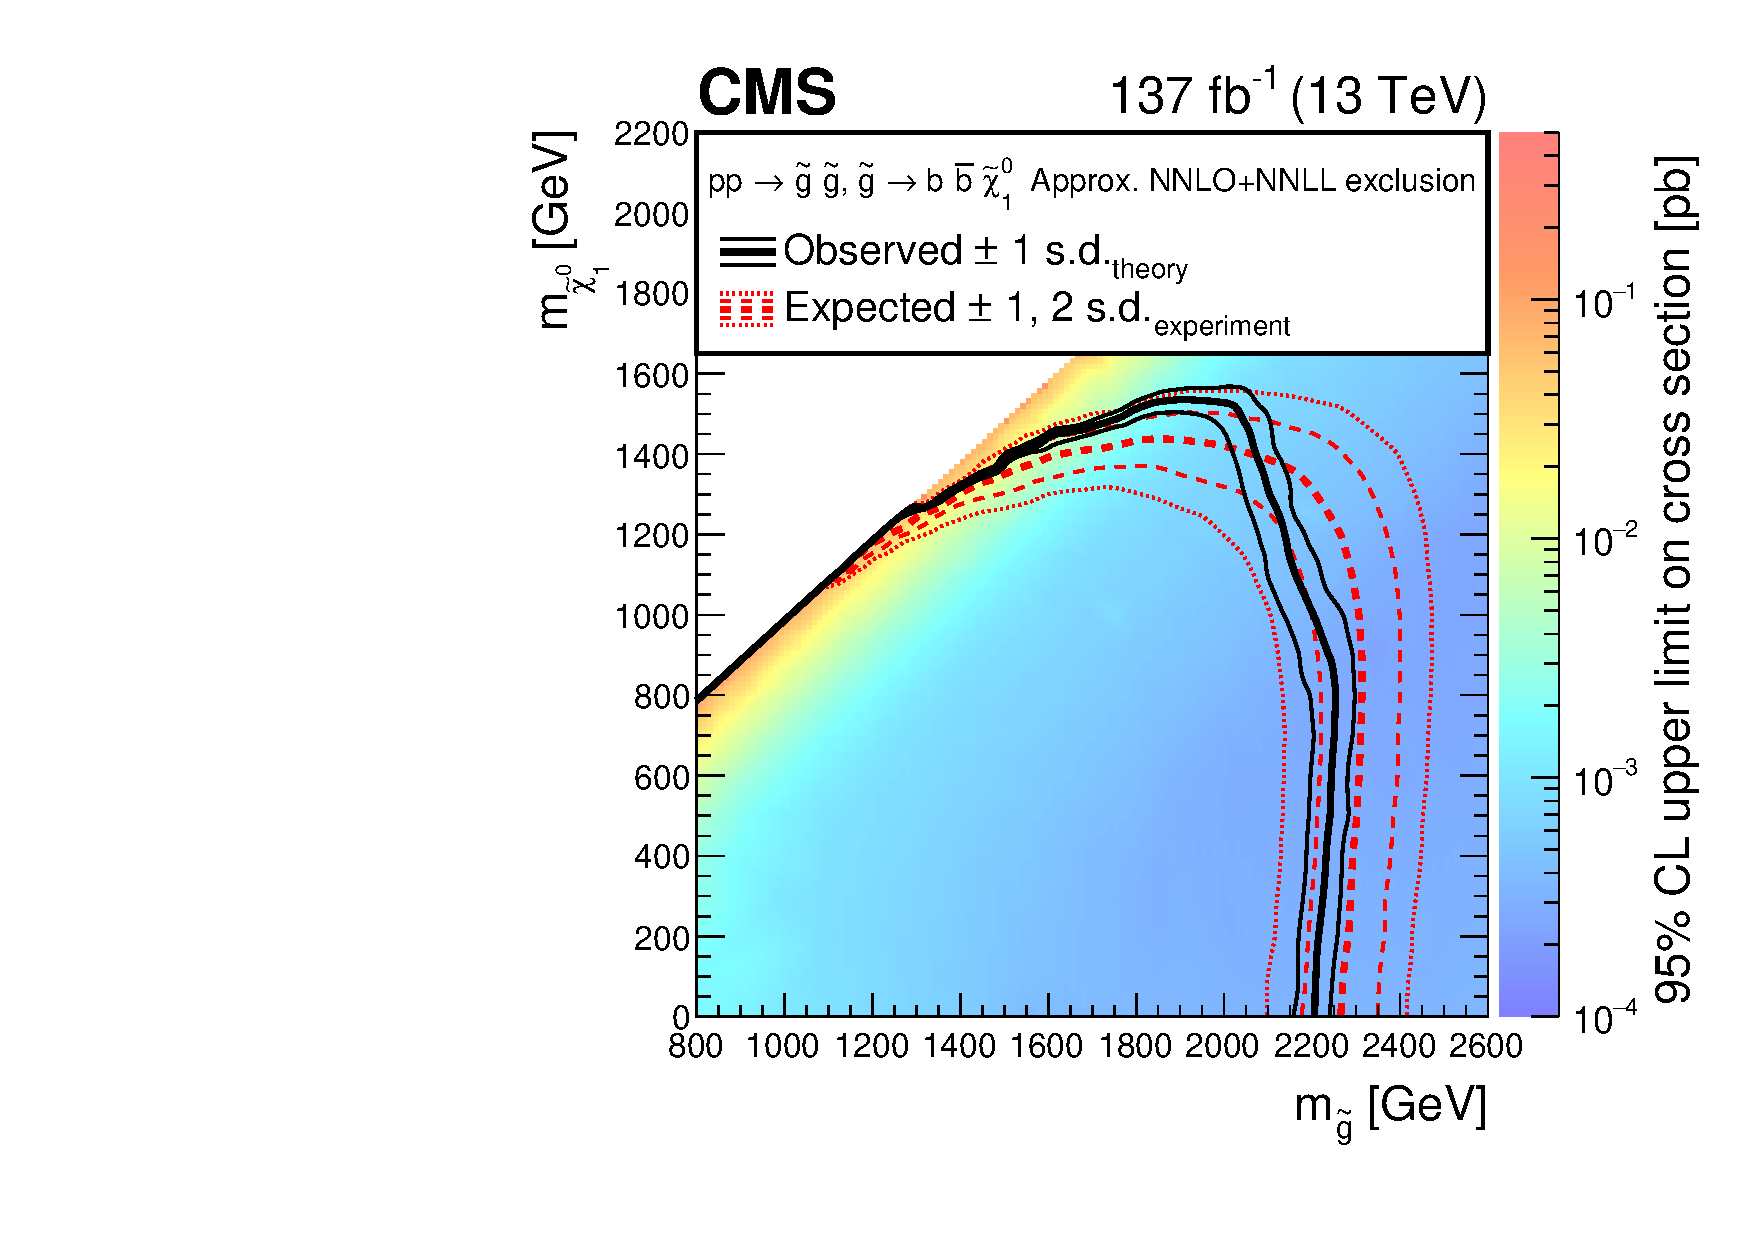
\includegraphics[width=0.48\textwidth]{figs/results/T1bbbbXSEC.pdf}
    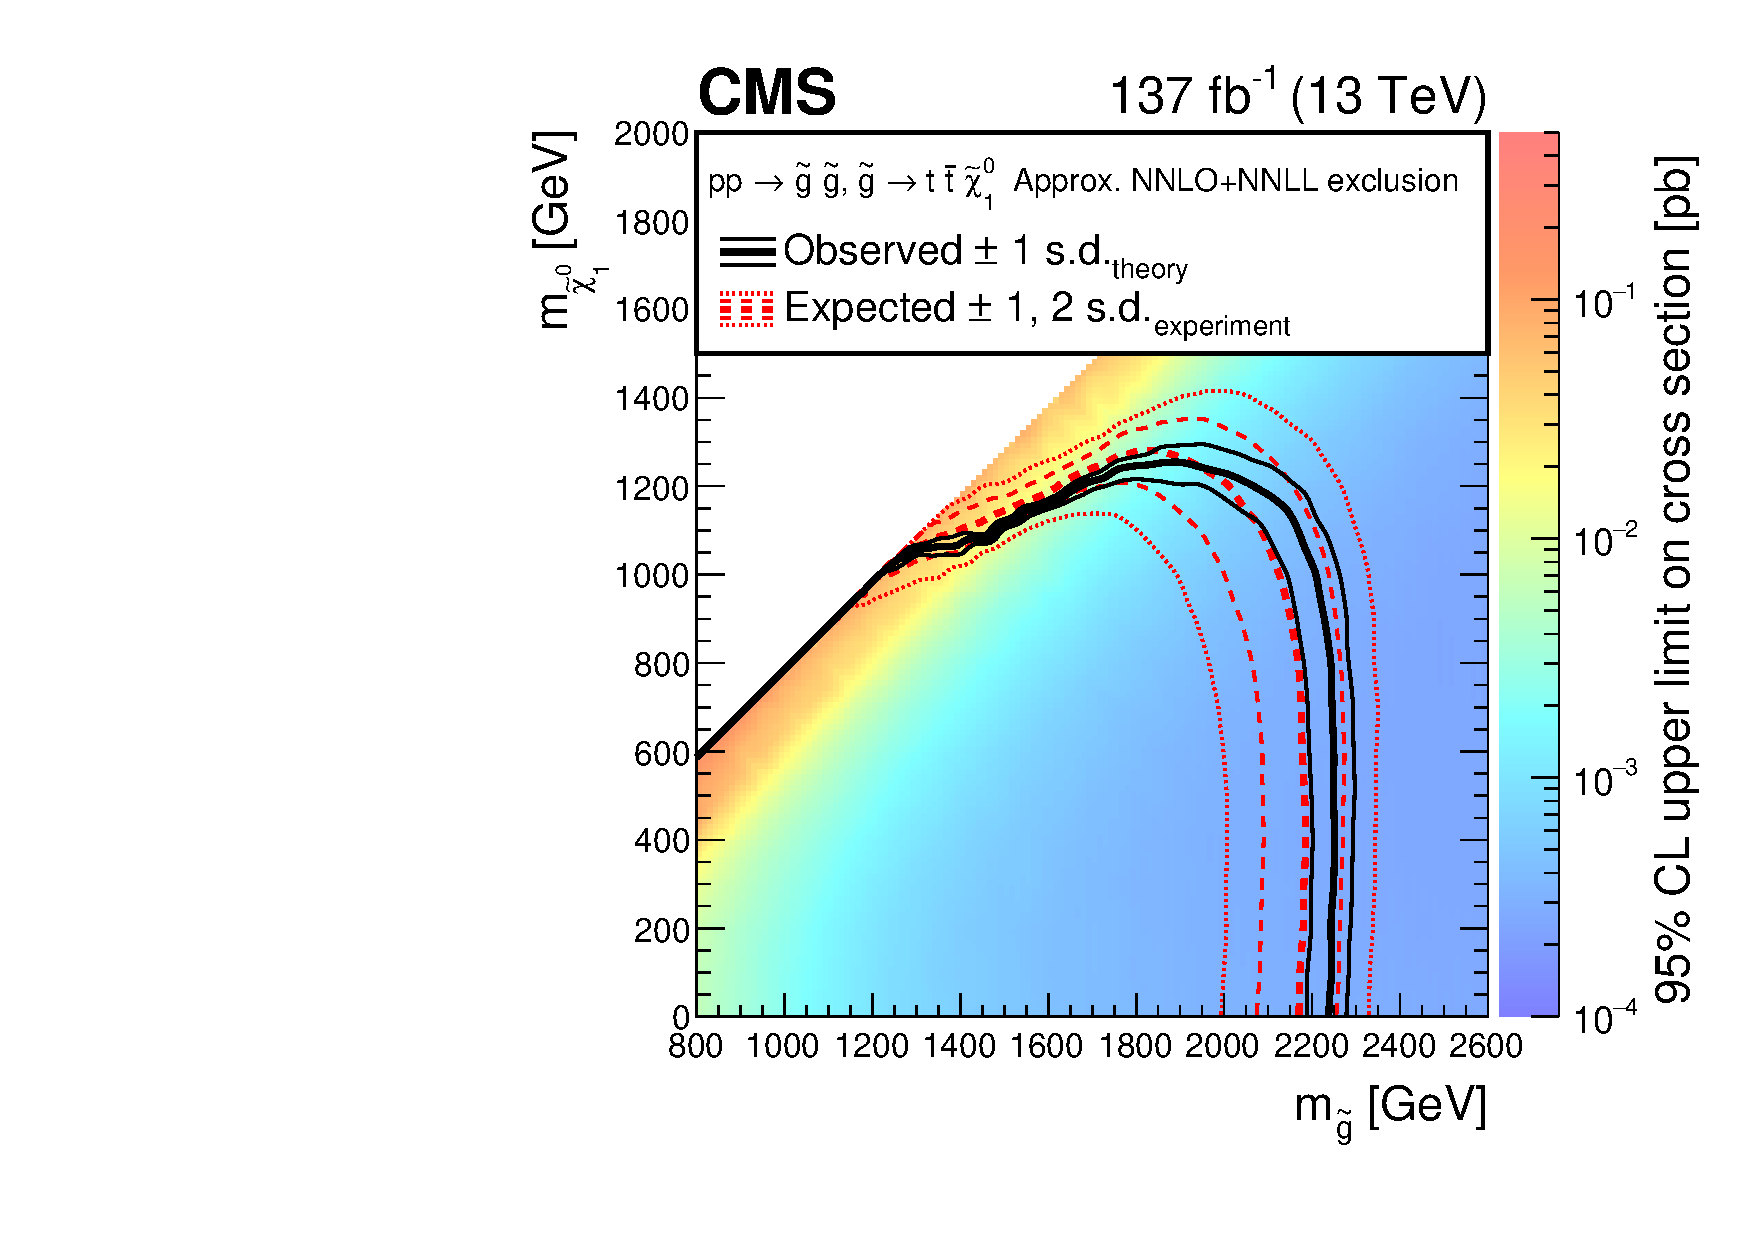
\includegraphics[width=0.48\textwidth]{figs/results/T1ttttXSEC.pdf}
    \caption{
    Exclusion limits at  95\% CL for
     direct gluino pair production where the gluinos decay to (left) bottom quarks and (right) top quarks.
      The area enclosed by the thick black curve represents the observed exclusion region,
      while the dashed red lines indicate the expected limits and
      their $\pm$1 and $\pm$2
      standard deviation ranges.
      The thin black lines show the effect of the theoretical
      uncertainties in the signal cross section.
      Signal cross sections are calculated at approximately NNLO+NNLL order in $\alpha_{\mathrm{s}}$~\cite{Beenakker:nnll},
      assuming unity branching fraction for the indicated decay.}
    \label{fig:t1x}
\end{figure}

\begin{figure}[htbp]
  \centering
    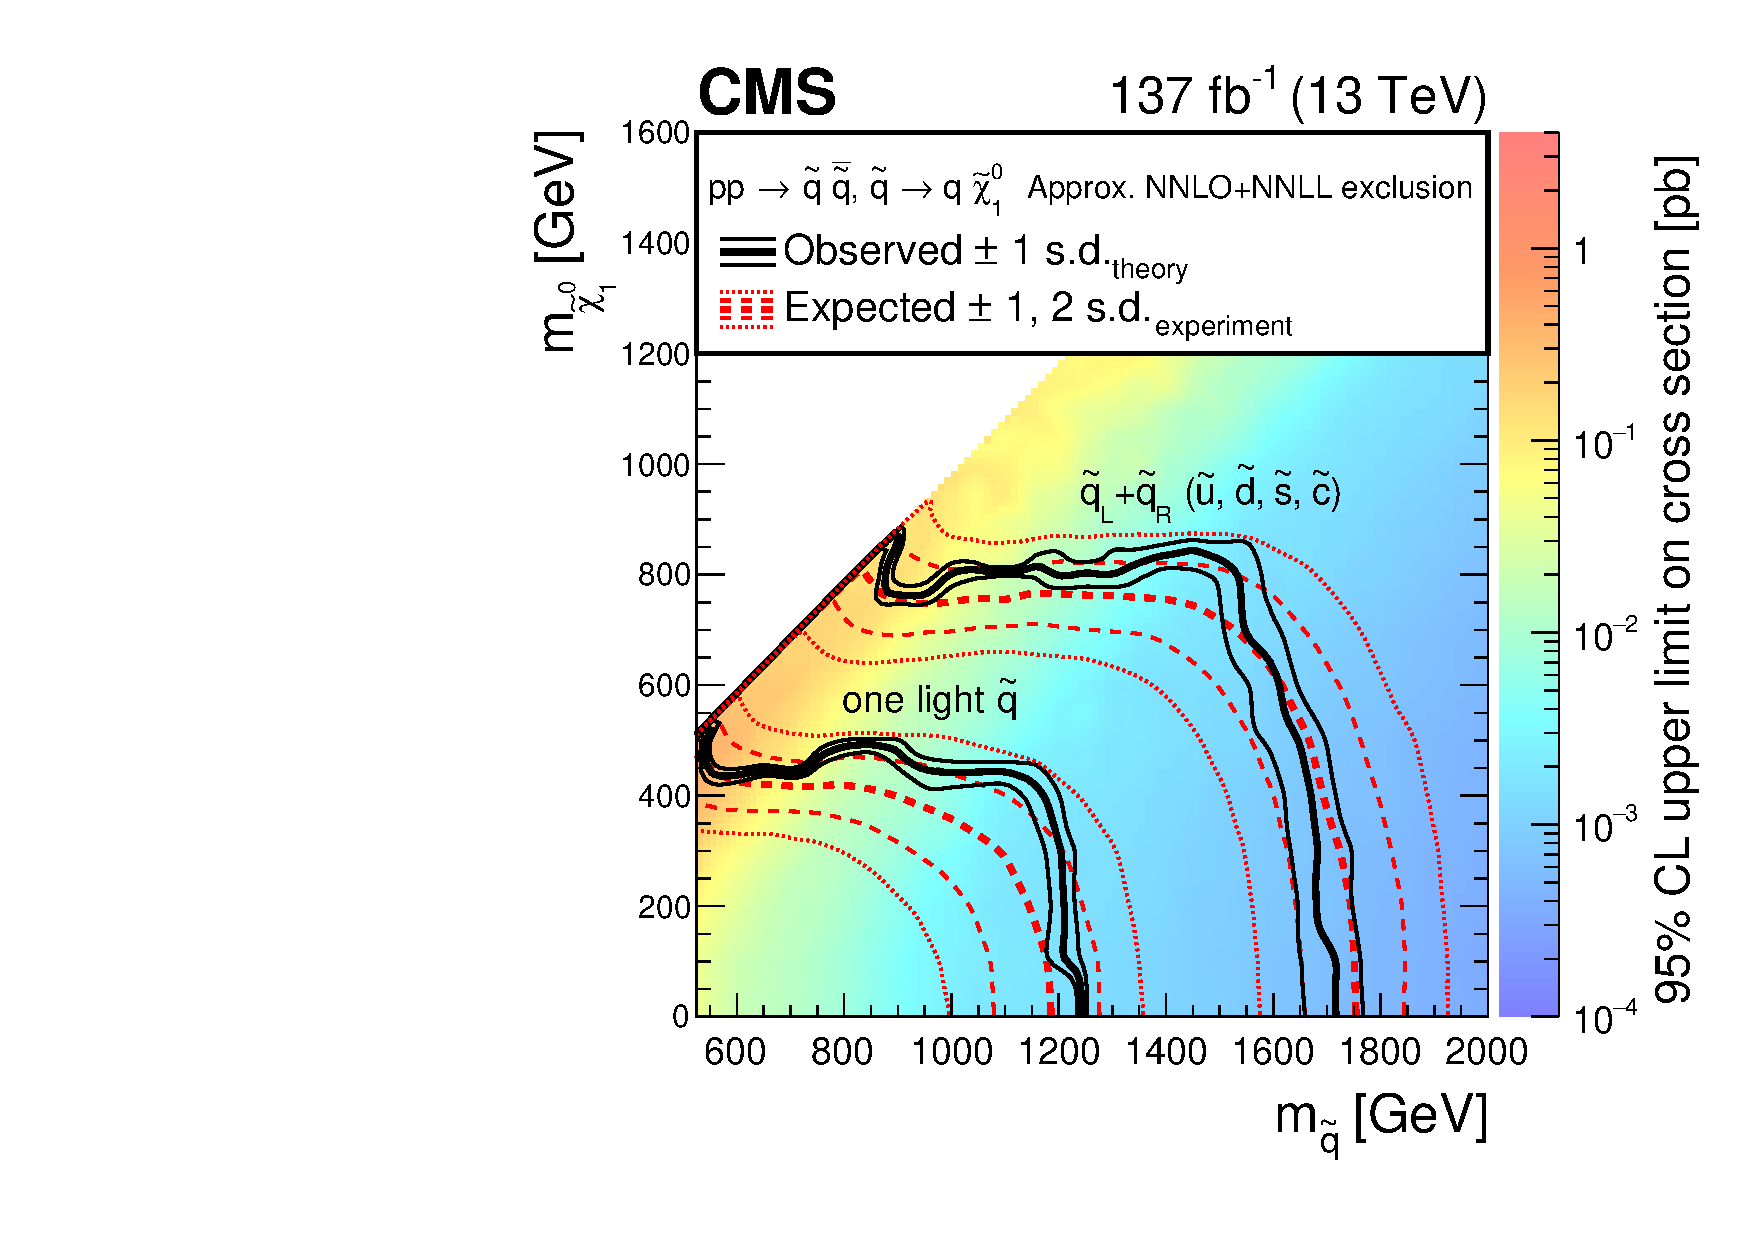
\includegraphics[width=0.48\textwidth]{figs/results/T2qq_XSEC_paperXSEC.pdf}
    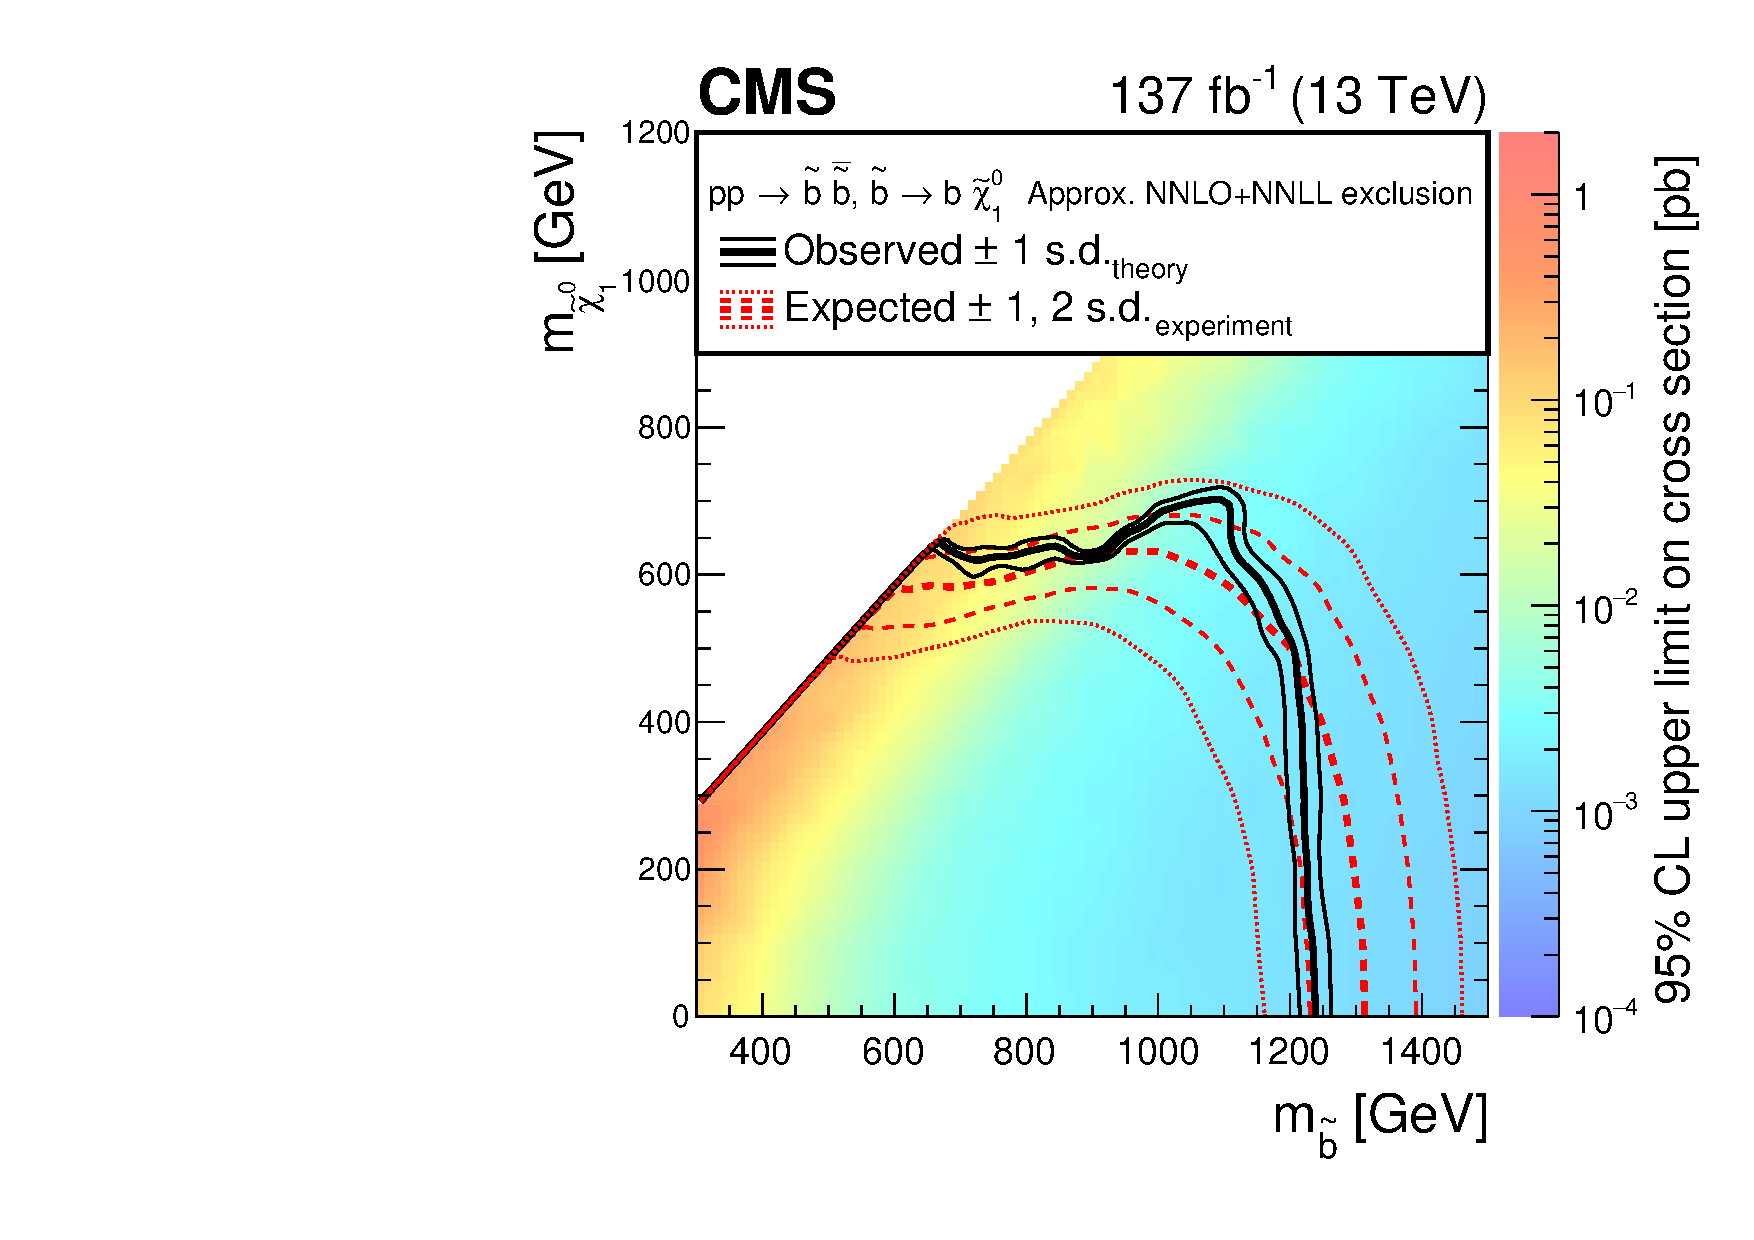
\includegraphics[width=0.48\textwidth]{figs/results/T2bb_XSEC_paperXSEC.pdf}
    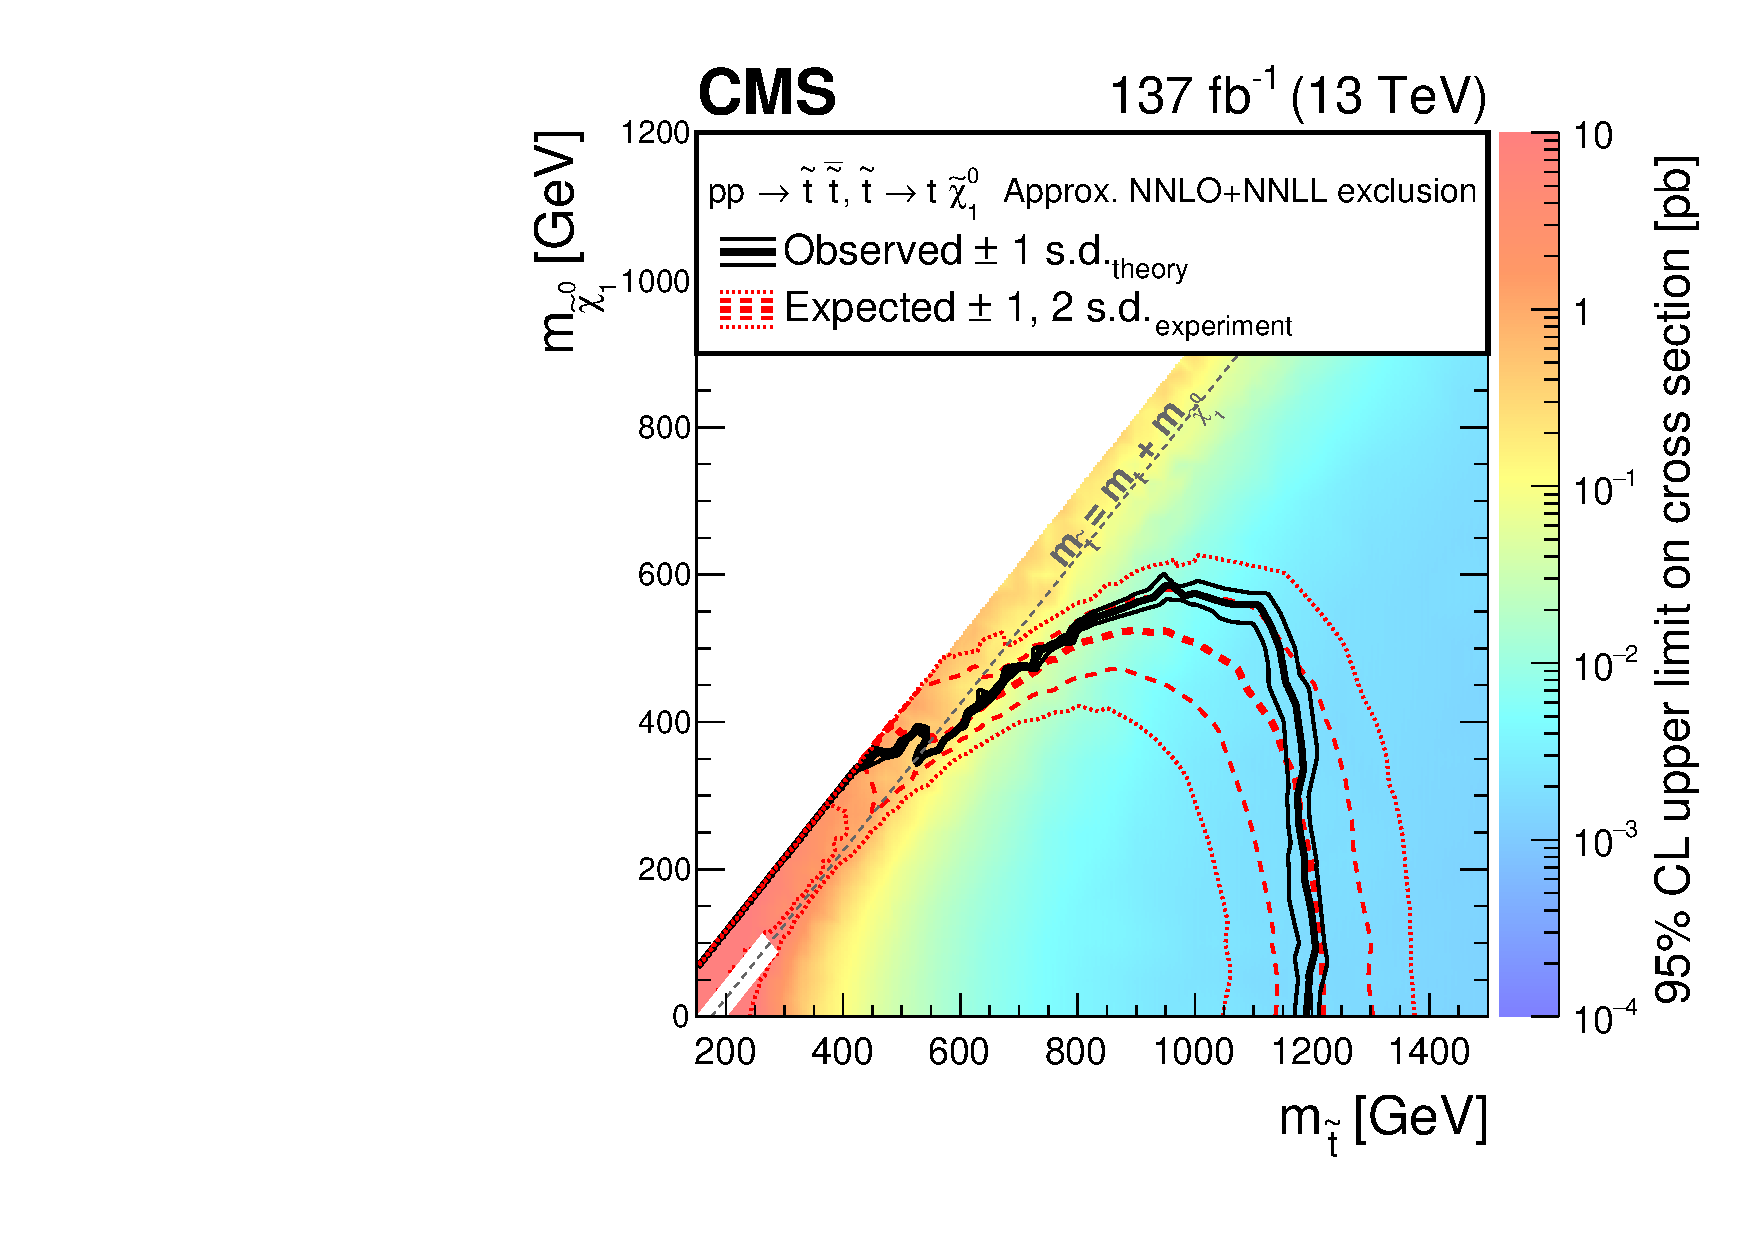
\includegraphics[width=0.48\textwidth]{figs/results/T2tt_XSEC_paperXSEC.pdf}
    \caption{
    Exclusion limit at 95\% CL for (upper left) light-flavor squark pair production, (upper right) bottom squark pair production,
    and (lower) top squark pair production.
      The area enclosed by the thick black curve represents the observed exclusion region,
      while the dashed red lines indicate the expected limits and
      their $\pm$1 and $\pm$2
      standard deviation ranges.
      The thin black lines show the effect of the theoretical
      uncertainties in the signal cross section.
      The white diagonal band in the top squark pair production exclusion limit corresponds to the region
      $\left|m_{\SQt}-m_{t}-m_{\lsp}\right|< 25\GeV$ and small $m_{\lsp}$. Here the efficiency of the selection
      is a strong function of $m_{\SQt}-m_{\lsp}$, and as a result the precise
      determination of the cross section upper limit is uncertain
      because of the finite granularity of the available
      MC samples in this region of the ($m_{\SQt}, m_{\lsp}$)  plane. In the same exclusion limit, the gray diagonal line corresponds to $m_{\SQt}=m_{t}+m_{\lsp}$.
      Signal cross sections are calculated at approximately NNLO+NNLL order in $\alpha_{\mathrm{s}}$~\cite{Beenakker:nnll},
      assuming unity branching fraction for the indicated decay.}
    \label{fig:t2x}
\end{figure}

\begin{figure}[htbp]
 \centering
   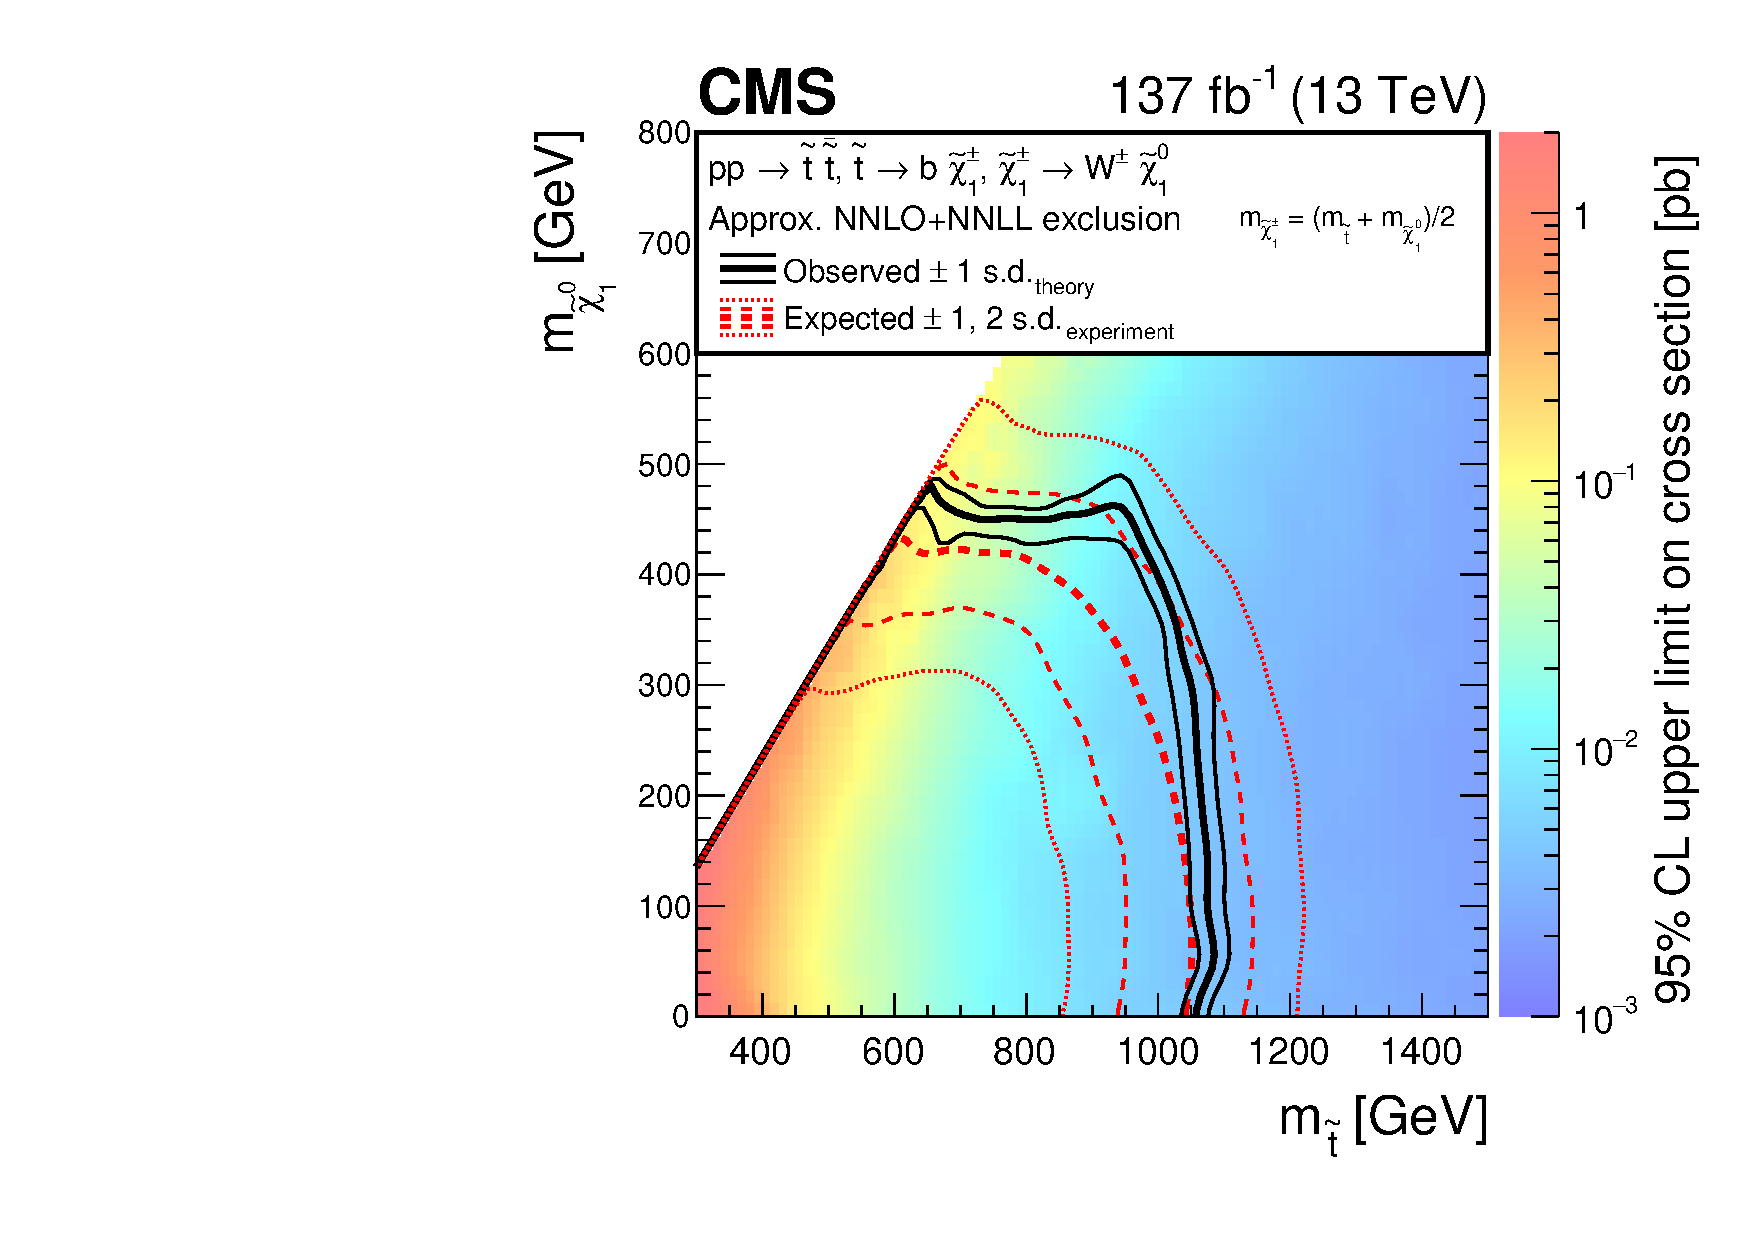
\includegraphics[width=0.49\textwidth]{figs/results/T2bW_XSEC_paperXSEC.pdf}
   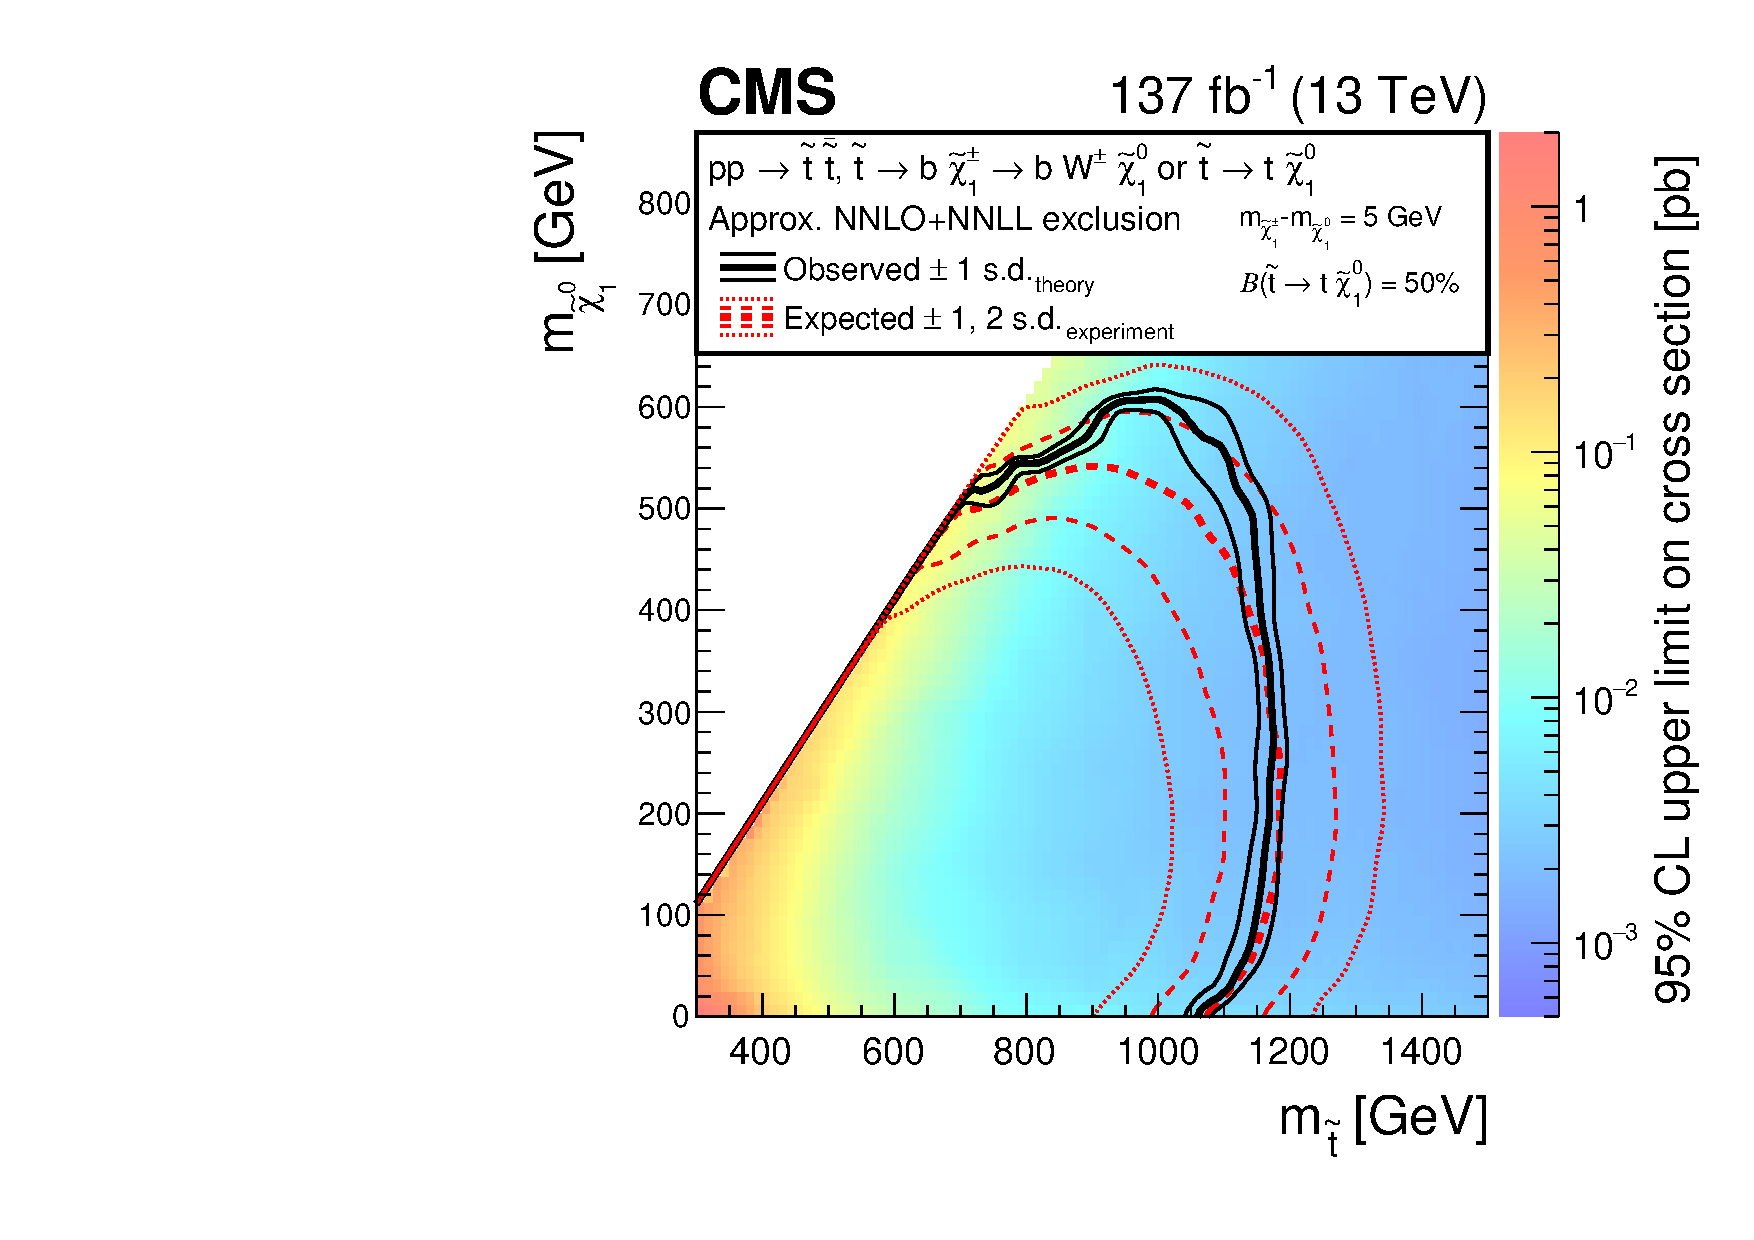
\includegraphics[width=0.49\textwidth]{figs/results/T2bt_XSEC_paperXSEC.pdf}
   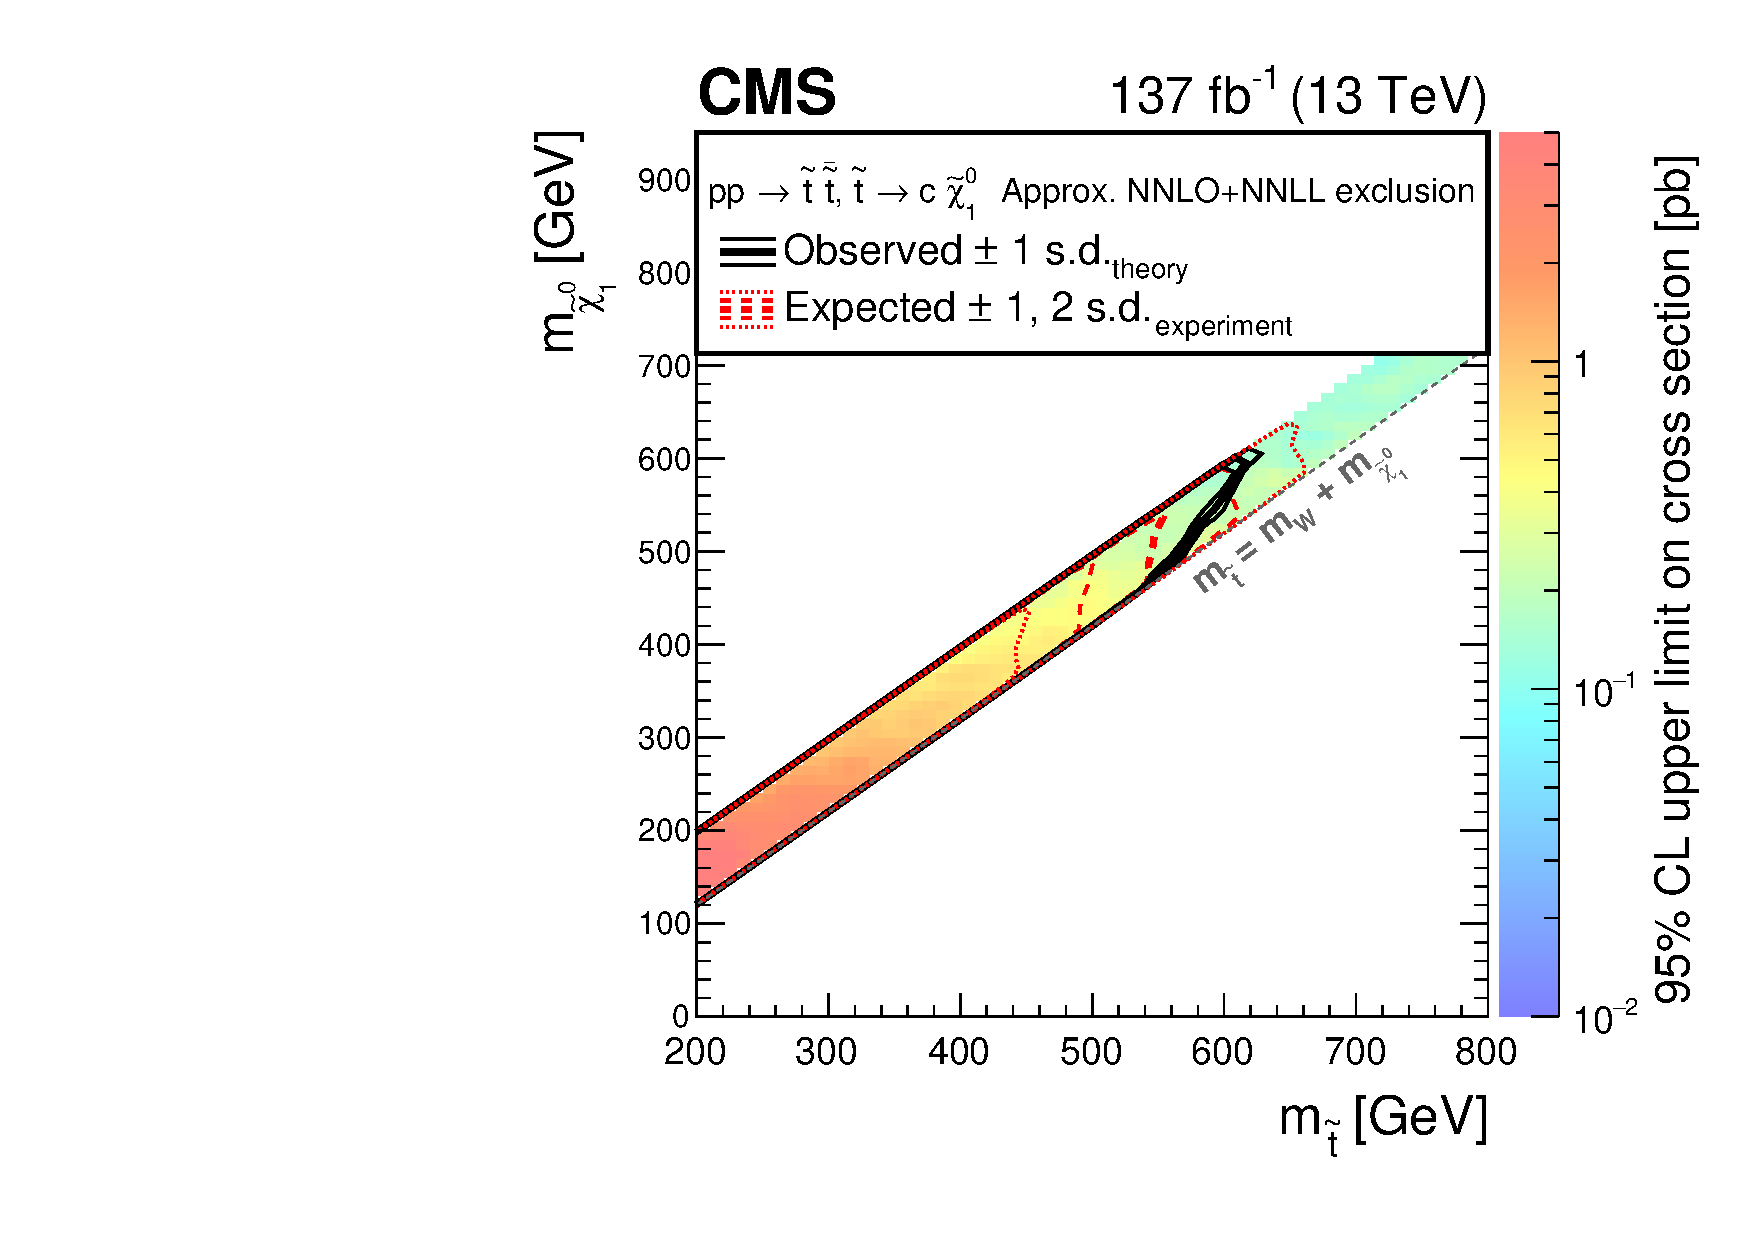
\includegraphics[width=0.49\textwidth]{figs/results/T2cc_XSEC_paperXSEC.pdf}
   \caption{Exclusion limit at 95\% CL for top squark pair production for different decay modes of the top squark.
     (Upper left) For the scenario where $pp\to\SQt\SQt\to b\bar{b}\chargino\chargino$, $\chargino\to W^{\pm}\lsp$,
     the mass of the chargino is chosen to be half way in between the masses of the top squark and the neutralino.
     (Upper right) A mixed-decay scenario, $pp\to\SQt\SQt$ with equal branching fractions for the top squark decays $\SQt\to t\lsp$
     and $\SQt\to b\charginoplus$, $\charginoplus\to W^{+}\lsp$,
     is also considered, with the chargino mass chosen such that
     $\Delta m\left(\chargino,\lsp\right) = 5\GeV$.
     (Lower) Finally, we also consider
     a compressed spectrum scenario where
     $pp\to\SQt\SQt\to c\bar{c}\lsp\lsp$. In this scenario, mass ranges are considered where $\SQt\to c\lsp$ branching fraction can be significant.
     The area enclosed by the thick black curve represents the observed exclusion region,
     while the dashed red lines indicate the expected limits and
     their $\pm$1  and $\pm$2
     standard deviation ranges.
     The thin black lines show the effect of the theoretical
     uncertainties in the signal cross section.
   }
   \label{fig:stop_other}
\end{figure}

\subsection {Mono-$\phi$ model}

The results of the inclusive \mttwo search are also interpreted in the context of a BSM scenario
where a colored scalar state $\phi$ is resonantly produced through coupling to quarks, and decays
to an invisible massive Dirac fermion $\psi$ and an SM quark. This is referred to as the mono-$\phi$
model. It has been proposed as an explanation of an excess in data in regions with
low jet multiplicities, identified in the context of a reinterpretation~\cite{Asadi1,Asadi2} 
of the results of the previous inclusive \mttwo search~\cite{CMS:mt22016} as well as of other
similar searches by the ATLAS~\cite{ATLAS:monojet,ATLAS:jetmet} and CMS~\cite{CMS:ra22016,CMS:jetmetwz} collaborations.
The diagram for the hypothetical process is shown in Fig.~\ref{fig:SMS_monophi}.


\begin{figure}[htbp]
  \centering
    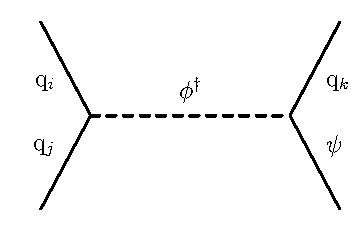
\includegraphics[width=0.3\textwidth]{figs/results/monoPhi.pdf}
    \caption{Diagram for the mono-$\phi$ model, where a colored scalar $\phi$ is resonantly produced, and then
      decays to an invisible massive Dirac fermion $\psi$ and a SM quark.}
    \label{fig:SMS_monophi}
\end{figure}

Figure~\ref{fig:monophi} shows the exclusion limits for the mono-$\phi$ model. Based on the LO cross
section calculation, we obtain mass limits as large as 1660 and 925\GeV on $m_\phi$ and $m_\psi$,
respectively. In this model, the analysis of Refs.~\cite{Asadi1,Asadi2} report best-fit parameters
$(m_\phi,m_\psi)=(1250,900)\GeV$ and product of the cross section times branching ratio of about
0.3 pb. For this mass point, we find a modest (1.1 standard deviation) excess, and we set an upper
limit on the product of cross section times branching ratio of about 0.6 (0.4 expected) pb.

\begin{figure}[htbp]
 \centering
   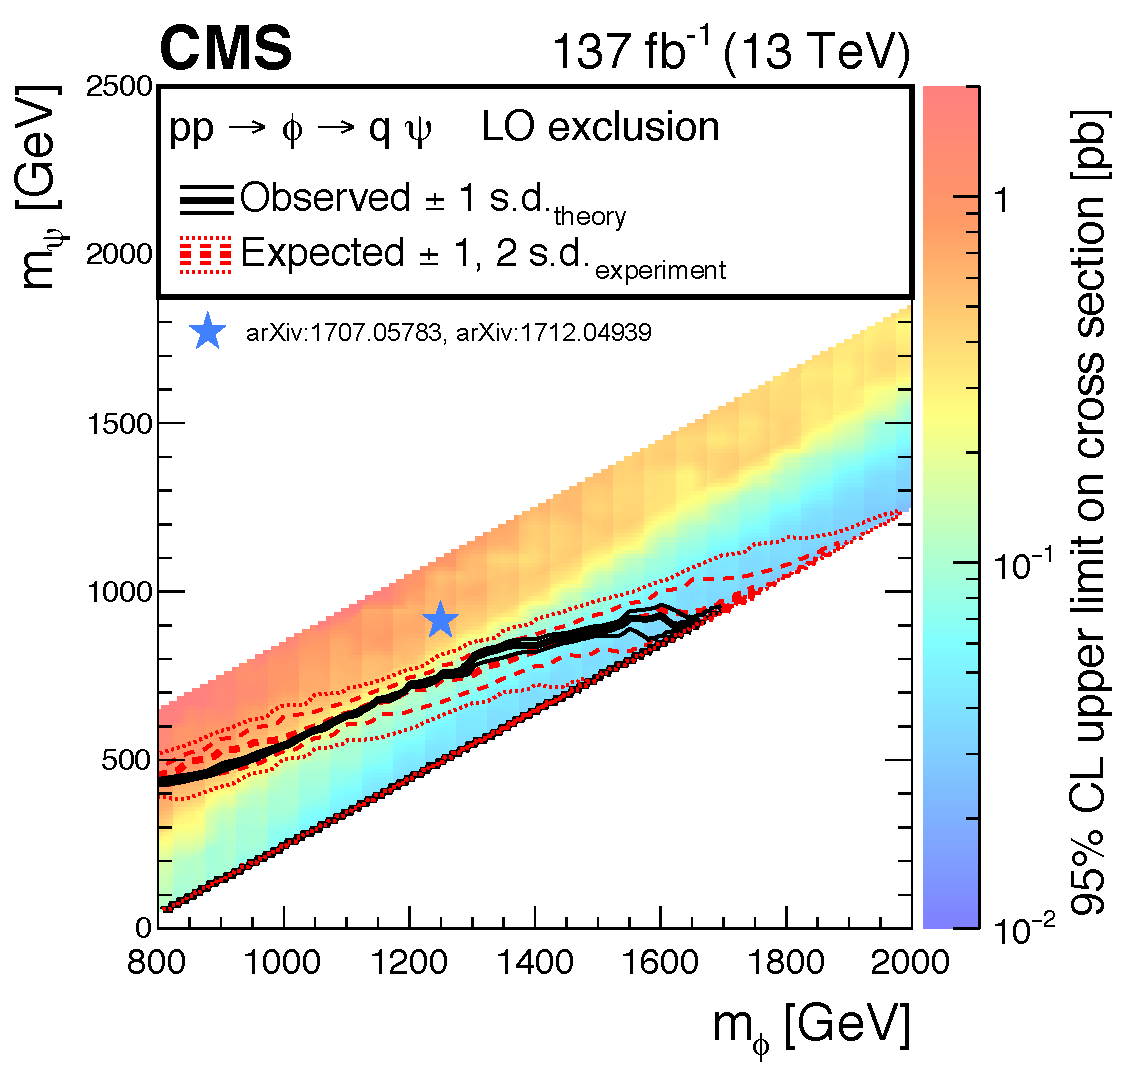
\includegraphics[width=0.49\textwidth]{figs/results/rpvMonoPhi_XSEC_paperXSEC_star_arxiv.pdf}
   \caption{Exclusion limit at 95\% CL for the mono-$\phi$ model.
     We consider the mass range where such a model could be interesting based on a
     reinterpretation of previous analyses~\cite{Asadi1,Asadi2}.
     The area enclosed by the thick black curve represents the observed exclusion region,
     while the dashed red lines indicate the expected limits and
     their $\pm$1 and $\pm$2 standard deviation ranges.
     The thin black lines show the effect of the theoretical
     uncertainties in the signal cross section.
     The blue star at $\left(m_{\phi},~m_{\psi}\right)=\left(1250,~900\right)\GeV$ indicates the best fit mass point reported in Refs.~\cite{Asadi1,Asadi2}.
     Signal cross sections are calculated at LO order
     in $\alpha_{\mathrm{s}}$.}
   \label{fig:monophi}
\end{figure}

\subsection {Leptoquark models}
\label{sec:interp_lq}

Finally, the search is interpreted in using models of leptoquark (LQ) pair production,
similarly to a previous reinterpretation~\cite{CMS:mt2LQ}. Leptoquarks, discussed in
Sec.~\ref{sec:leptoquarks}, are hypothetical particles that couple quarks and leptons. As they
are necessarily colored, they also couple to gluons, giving the four main production
modes shown in Fig.~\ref{fig:SMS_LQ}.

\begin{figure}[htbp]
  \centering
    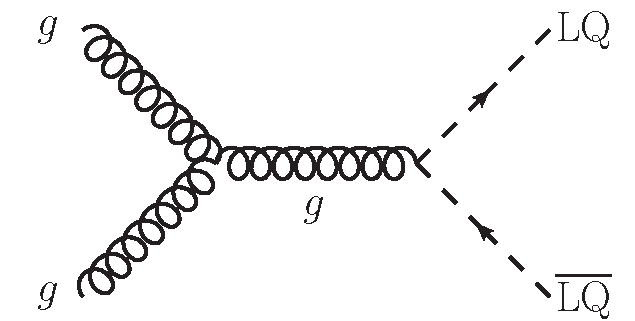
\includegraphics[width=0.24\textwidth]{figs/results/LQdiagram_a.pdf}
    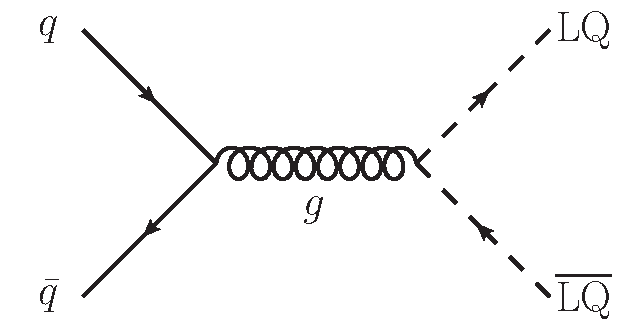
\includegraphics[width=0.24\textwidth]{figs/results/LQdiagram_b.pdf}
    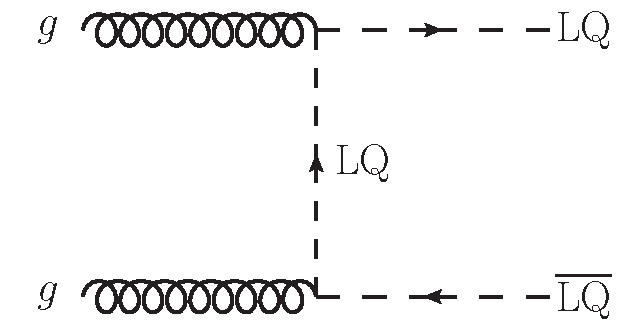
\includegraphics[width=0.24\textwidth]{figs/results/LQdiagram_c.pdf}
    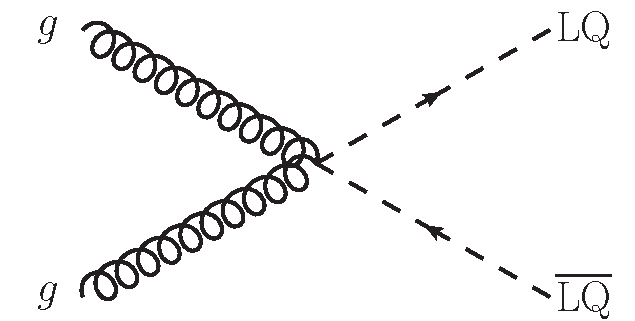
\includegraphics[width=0.24\textwidth]{figs/results/LQdiagram_d.pdf}
    \vspace{3mm}
    \caption{Diagrams for LQ pair production.}
    \label{fig:SMS_LQ}
\end{figure}

In the case of scalar leptoquarks (\lqs), the kinematics are identical to the
pair production of squarks, where each squark decays to a quark and \lsp with $m_\lsp=0$.
Differences in kinematic distributions introduced by vector leptoquarks (\lqv) are negligible,
at least for the variables relevant to this analysis. Hence, the same signal simulation is
used as for the pair production of squarks, with $m_\lsp$ set to 0, and rescaled to the
theoretical LQ pair production cross section.

Figure~\ref{fig:lq} shows the 95\% CL exclusion limits on the cross section times branching ratio
of $\mrm{LQ}\to q\nu$, as a function of LQ mass, where $q$ is either a light-flavor quark, bottom quark, or top
quark. Theory curves are the cross sections assuming 100\% branching fraction to the relevant quark-neutrino pair,
except for the pink curve in the bottom plot which assumes $\mathcal{B}(\lqv\to t\nu)=50\%$ and
$\mathcal{B}(\lqv\to b\tau)=50\%$, corresponding to a proposed explanation~\cite{Buttazzo:bphys} of various flavor
physics anomalies.

Table~\ref{tab:lim_lq} summarizes the limits on the masses of the leptoquarks excluded for the considered scenarios.
These results extend the constraints on LQ masses by up to 200\GeV with respect to the limits of Ref.~\cite{CMS:mt2LQ},
providing the most stringent constraints to date on models of LQ pair production.

\begin{figure}[htbp]
 \centering
   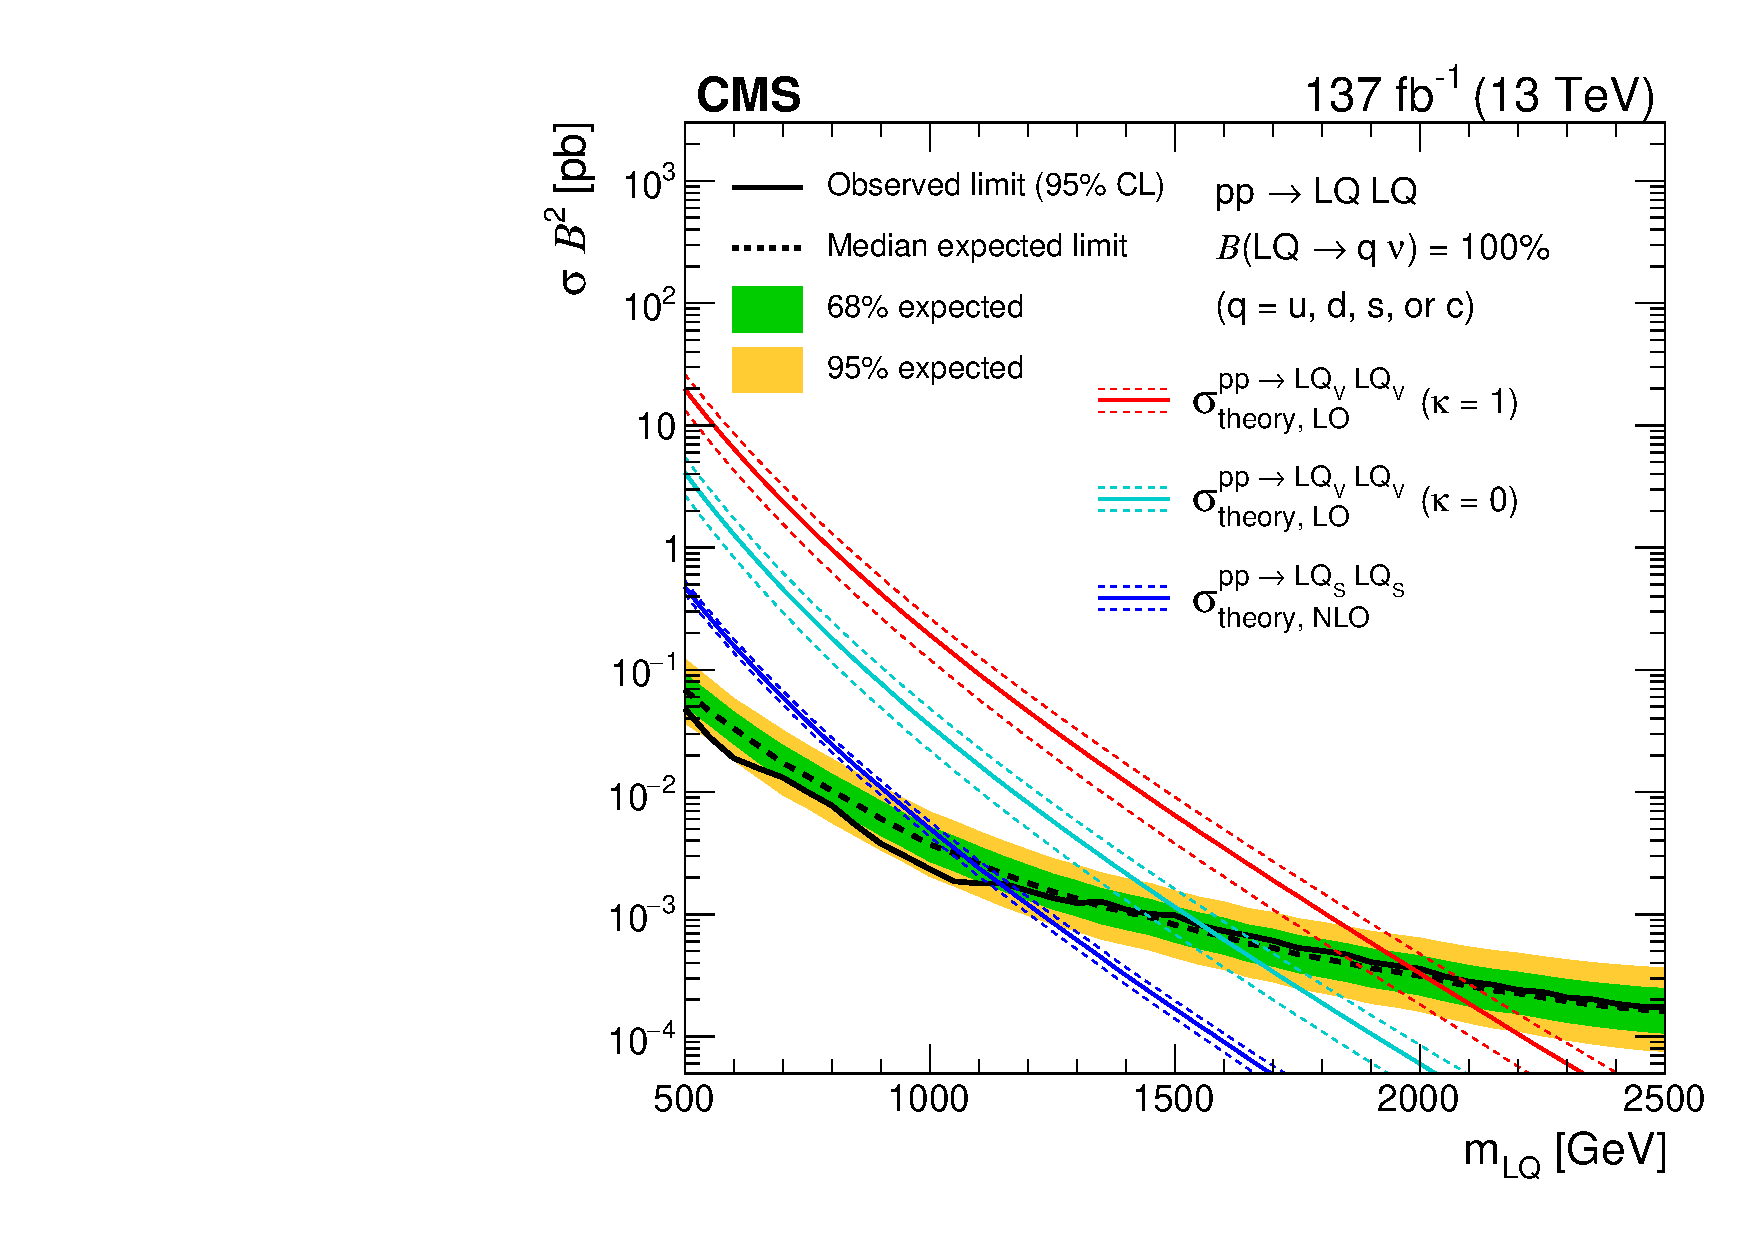
\includegraphics[width=0.48\textwidth]{figs/results/LQ_q.pdf}
   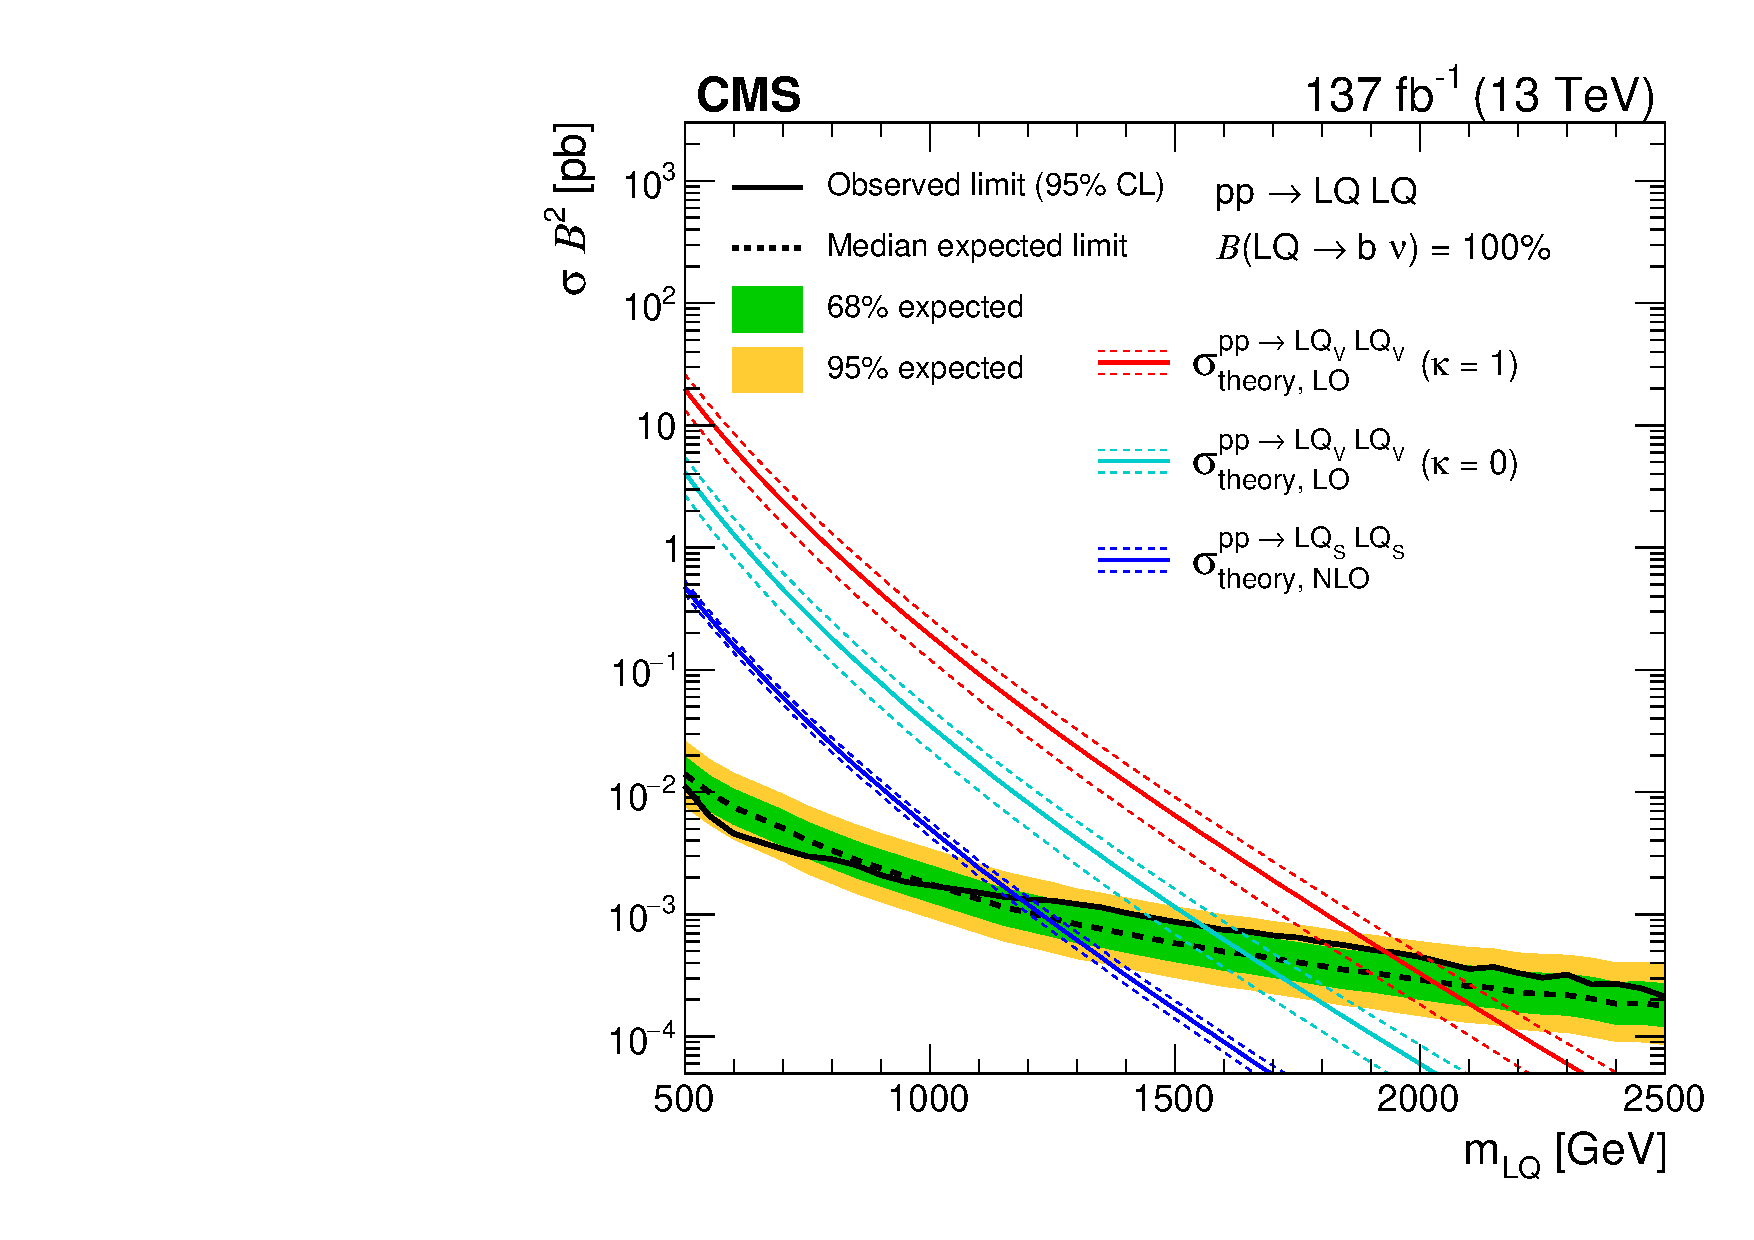
\includegraphics[width=0.48\textwidth]{figs/results/LQ_b.pdf}
   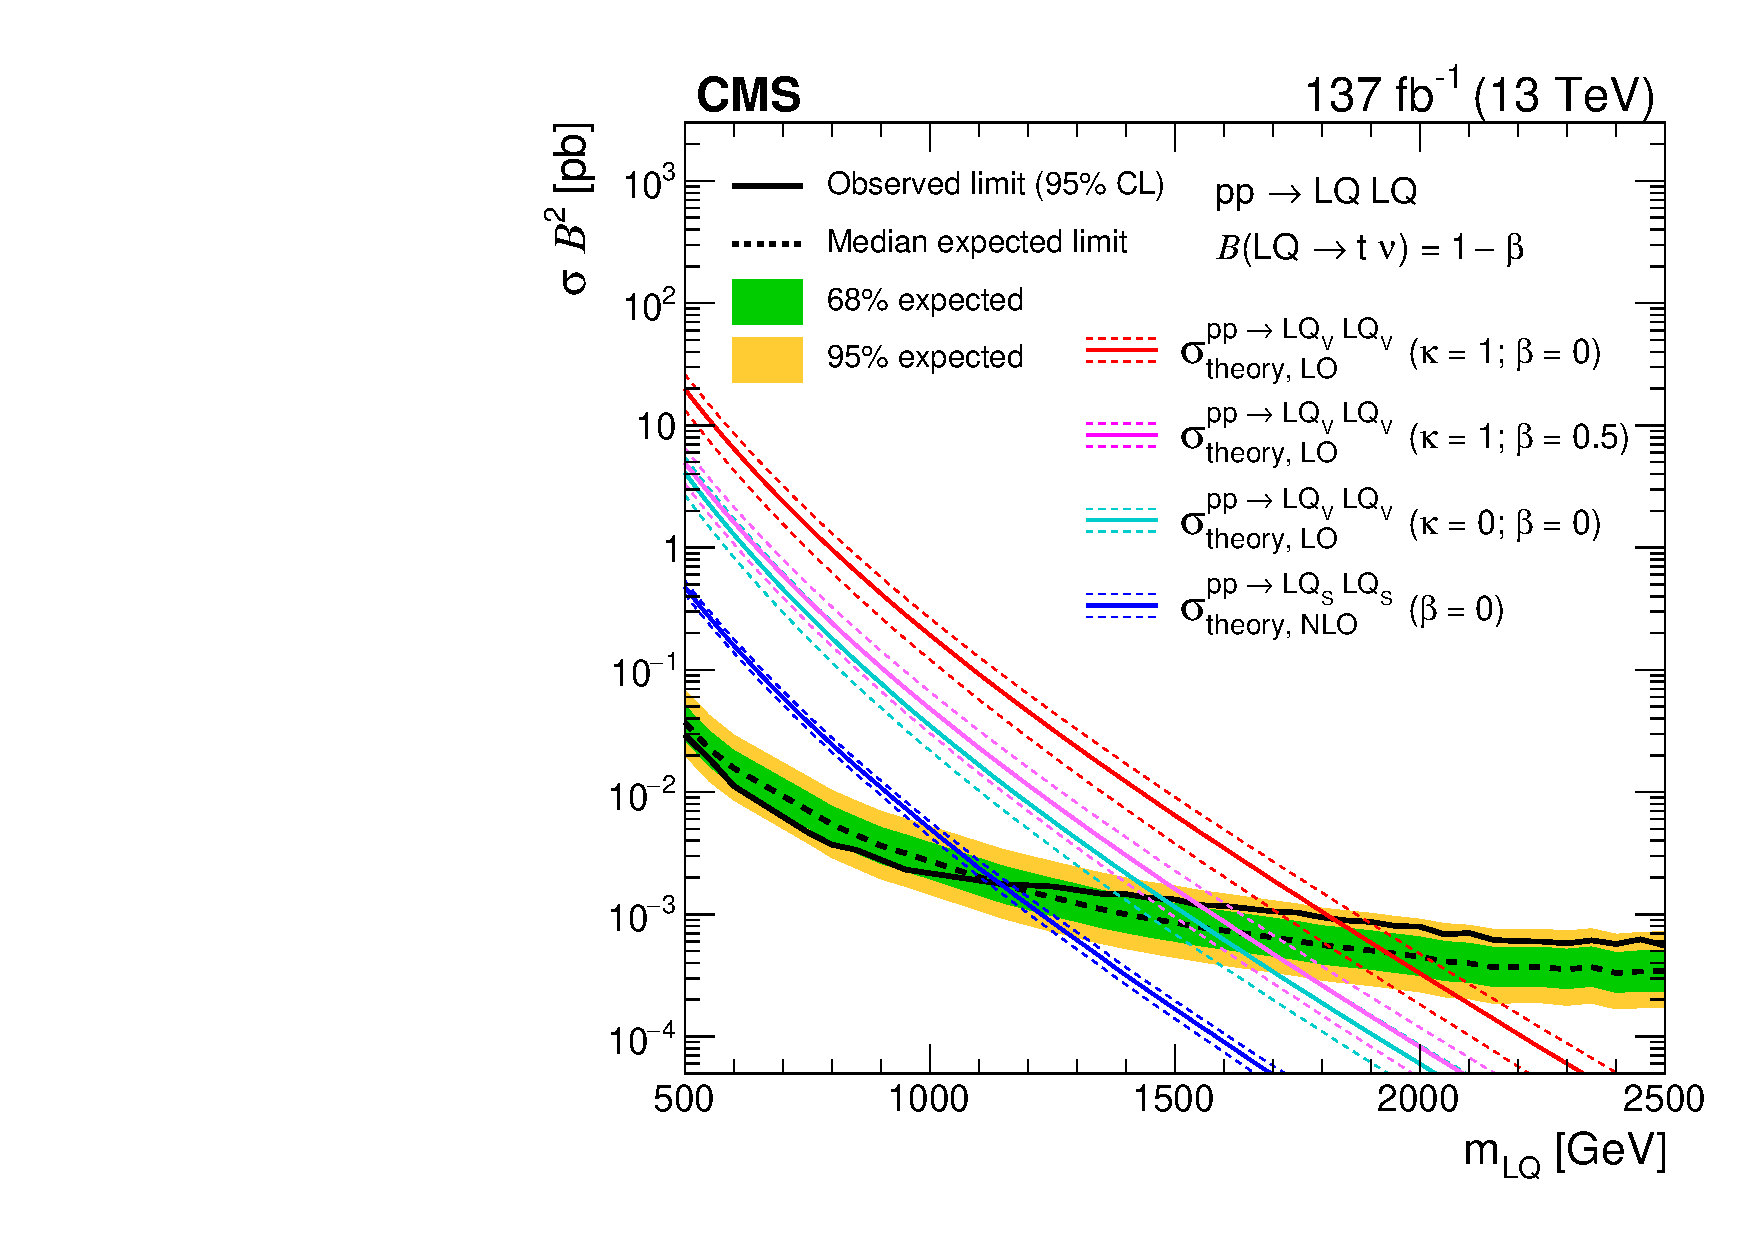
\includegraphics[width=0.48\textwidth]{figs/results/LQ_t.pdf}
   \caption{The 95\% CL upper limits on the production cross sections as a function of LQ mass
for LQ pair production decaying with 100\% branching fraction ($\mathcal{B}$) to a neutrino and (upper left) a light quark
(one of $u,\;d,\;s,\;\text{or}\;c$),
(upper right) a bottom quark, or (lower) a top quark.
The solid (dashed) black line represents the observed (median expected) exclusion.
The inner green (outer yellow) band indicates the region containing 68 (95)\%
of the distribution of limits expected under the background-only hypothesis.
The dark blue lines show the theoretical cross section for \lqs pair production with its uncertainty.
The red (light blue) lines show the same for \lqv\ pair production assuming $\kappa = 1$ (0).
(Lower) Also shown in magenta is the product of the theoretical cross section and the square of the branching fraction ($\sigma \mathcal{B}^{2}$),
for vector LQ pair production assuming $\kappa = 1$ and a 50\% branching fraction to $t\nu_\tau$, with the remaining 50\% to $b\tau$.
Signal cross sections are calculated at NLO (LO) in $\alpha_{\mathrm{s}}$ for scalar (vector) LQ pair production.}
   \label{fig:lq}
\end{figure}


\begin{table}[htb]
  \caption{Summary of the observed 95\% CL exclusion limits on the masses of LQs for the considered scenarios. The columns show scalar or vector LQ with the choice of $\kappa$,
while the rows show the LQ decay channel. For mixed-decay scenarios, the assumed branching fractions ($\mathcal{B}$) are indicated.
    \label{tab:lim_lq}}
\centering
\begin{tabular}{l|c|c|c}
\hline
 & \lqs  & $\lqv,~\kappa=1$ & $\lqv,~\kappa=0$ \\
 & mass [\GeV] & mass [\GeV] & mass [\GeV] \\
\hline\hline
$\mathrm{LQ}\to q\nu~\left(q=u,\;d,\;s,\;\text{or}\;c\right)$ & 1140 & 1980 & 1560\\
$\mathrm{LQ}\to b\nu$ & 1185 & 1925 & 1560 \\
$\mathrm{LQ}\to t\nu$ & 1140 & 1825 & 1475\\
$\mathrm{LQ}\to\left\{
\begin{tabular}{l}
$t\nu~\left(\mathcal{B}=50\%\right)$\\                                                                                                                                                                                                                                       
$b\tau~\left(\mathcal{B}=50\%\right)$                                                                                                                                                                                                                                         
\end{tabular}\right.$
& --- & 1550 & 1225 \\
\hline
\end{tabular}
\end{table}
